\documentclass[12pt]{article}
\usepackage[utf8]{inputenc}
\usepackage{amsmath}
\usepackage{mathrsfs}
\usepackage{amssymb}
\usepackage{amsfonts}

\DeclareMathOperator{\logit}{logit}
\DeclareMathOperator*{\argmax}{arg\,max}
\DeclareMathOperator*{\argmin}{arg\,min}
\newcommand{\red}[1]{\textcolor{red}{#1}}
\newcommand{\blue}[1]{\textcolor{blue}{#1}} 

\usepackage[
    a4paper,
    left = 2.5cm,
    right = 2.5cm,
    top = 2.5cm,
    bottom = 2.5cm
]{geometry}

\usepackage{graphicx}
\usepackage{subcaption}
\usepackage{booktabs}
\usepackage{adjustbox}
\usepackage{placeins}
\usepackage[headings]{fullpage}
\usepackage{xcolor}
\usepackage{hyperref}
\usepackage{fancyhdr}
 %For aligned formulas
 \usepackage{IEEEtrantools}
\usepackage{listings} %Source code listings https://en.wikibooks.org/wiki/LaTeX/Source_Code_Listings

% \lstset{
%     language=R, %You can always set to another language
%     breaklines,
%     deletekeywords={category},
%     basicstyle=\ttfamily\footnotesize,
%     otherkeywords={!,!=,~,\$,*,\&,\%/\%,\%*\%,\%\%,<-,<<-},
%     literate={~}{$\sim$}1 {<-}{{$\gets$}}1
% }

\usepackage[
    backend=biber,
    style=apa,
    maxcitenames=2,
    mincitenames=1,
    sorting=ynt
    ]{biblatex}
\addbibresource{bibfile.bib}

\setlength{\headheight}{15pt}
\pagestyle{fancy}
\fancyhf{}
\rhead{Odole, Cunha, and Murthy} % Fill in your name
%\lhead{Bayesian Statistics \& Probabilistic Machine Learning---Project Report}
\rfoot{Page \thepage}


\begin{document}

\begin{titlepage}
        \centering % Center all text
        \vspace*{\baselineskip} % White space at the top of the page
        
        {\huge YOUR TITLE}\\[0.2\baselineskip] % Title
        
        
        \vspace*{\baselineskip}
        
        {\Large --- Project Report ---\\
          Advanced Bayesian Data Analysis\\[\baselineskip]} % Tagline(s) or further description
        \vspace*{\baselineskip}
        
        {\LARGE Eldaleona Odole,  Leonor Cunha, and Anarghya Murthy\\[\baselineskip]} % Editor list  
        
        \vspace*{\baselineskip}

        \vfill
        
        \today \par % Location and year
        
        \vspace*{\baselineskip}

        {\itshape TU Dortmund University\par} % Editor affiliation
    \end{titlepage}

\clearpage

% \section{Template}
% This is a template for the project report in the course Advanced Bayesian Data Analysis.
% Fill in your title and names for the title page and header and follow the general structure. You don't have to use multiple chapters or sections at all for this short report, but if you do, don't go further than subsections--- \textcite{feynman1963lnphysics} didn't need to\ldots

% Some examples on how to use \LaTeX{} are shown below. If you want to reference something, you can do it as so:
% \textcite{mcelreath2016statistical}.

% \subsection{Images}
% \begin{figure}
%     \begin{center}
%     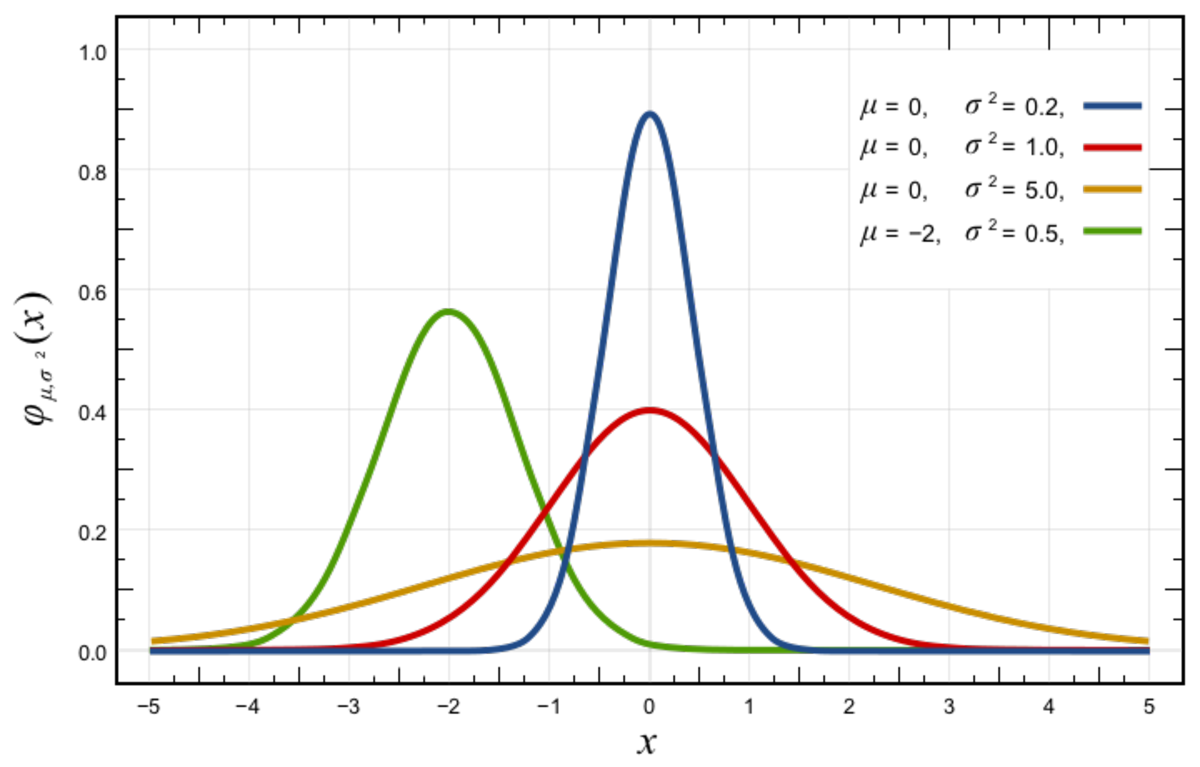
\includegraphics[width=0.5\textwidth]{figures/Normal_Distribution_PDF.pdf} %try to never force a figure placement
%     \caption{Probability density function for the Normal distribution. The red curve is the standard normal distribution. [By Inductiveload - self-made, Mathematica, Inkscape, Public Domain, \url{https://commons.wikimedia.org/w/index.php?curid=3817954}]}
%     \label{fig:normal_sample}
%     \end{center}
% \end{figure}

% This is an example for how to insert images into your document. When talking about a figure, you should always point out which one you mean, i.e., ``As you can see in Figure~\ref{fig:normal_sample}.''

% \subsection{Tables}
% A table has a caption \textit{above} the table as in Table~\ref{tab:my_label}.

% \begin{table} %You can place [h] immediately after \begin{table} to force the placement of the table. Generally speaking never do that---LaTeX usually places them in a sane way!
%     \centering
%     \caption{My caption.}
%     \label{tab:my_label}
%     \begin{tabular}{c|l} % l, r, and c justified inside cells.
%         \hline
%          Poisson & $\lambda$ \\ % Always end a line with \\
%          Normal &  $\mu$ and $\sigma$\\ 
%         \hline
%     \end{tabular}
% \end{table}

% \subsection{Formulas}
% This is a small example for how to include formulas into your document. $a^2 + b^2 = c^2$ will inline a formula, while
% $$c \leq a + b$$
% will give the formula its own line.

% \subsection{Formulas}
% You also might want to write out models:

% {\footnotesize % you align formulas using & 
% \begin{IEEEeqnarray*}{rCl}
% \mathrm{L}_i & \sim & \mathrm{Binomial}(n_i,p_i)\\
% \mathrm{logit}(p_i) & = & \alpha_{\mathrm{SUBJECT}[i]} + (\beta_P + \beta_{PC}C_i)P_i\\
% \alpha_{\mathrm{SUBJECT}} & \sim & \mathrm{Normal}(0,10) \\
% \beta_P & \sim & \mathrm{Normal}(0,10)\\
% \beta_{PC} & \sim & \mathrm{Normal}(0,10)
% \end{IEEEeqnarray*}
% }


% \subsection{Source code}
% Of course, formatting source code is always nice.
% \begin{lstlisting}
% m <- map(
%     alist(
%         height ~ dnorm(mu, sigma),
%         mu <- a + b*weight,
%         a ~ dnorm(0, 100),
%         b ~ dnorm(0, 10),
%         sigma ~ dunif(0, 50) 
%     ), 
%     data=d2)
% \end{lstlisting}

% \subsection{Math fonts}
% Different math fonts are also available to you:

% $\mathrm{ABCDE abcde 1234}$

% $\mathit{ABCDE abcde 1234}$

% $\mathnormal{ABCDEabcde1234}$

% $\mathcal{ABCDE abcde 1234}$

% $\mathscr{ABCDE abcde 1234}$

% $\mathfrak{ABCDE abcde 1234}$

% $\mathbb{ABCDE abcde 1234}$



\thispagestyle{empty} % Prevents the header and footer from being displayed on the title page
\newpage

\tableofcontents
\newpage


\section{Introduction}
 

% In this report we aim to answer the question "How does urbanization of a US House District affect the resulting party that is elected?". 

In this report we aim to investigate the relationship between urbanization and partisanship voting outcomes. Put more concretely we want to answer the question; "How does urbanization of a particular US House distrcit affect the resulting party that is elected?". First we our motivation and important background information about the US election system. 
We then discuss briefly our modeling approach before looking at other literature trying to understand the relationship between urbanization and voting outcomes. 
Next we discuss our dataset, which is a combination of four different datasets, followed by a brief explaination of our codebase. 
We then discuss the set up of our four models in detail, followed by a discussion of the priors and our reasoning behind them. We then go into the results of our models and their convergence diagnostics. Next we use both graphical and numerical methods to compare our models. Finally we perform a prior sensitivity analysis before concluding with limitations, improvements and reflections. 


\begin{figure}[!ht]
	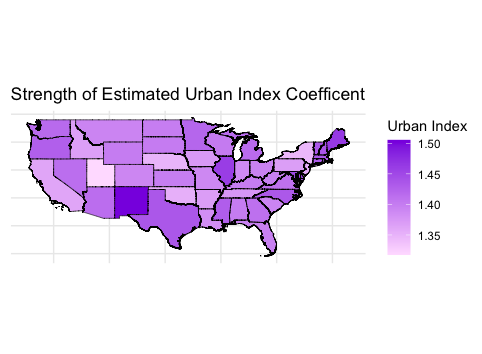
\includegraphics[width=\linewidth]{figures/beginning_image.png}
	
	\caption{A map of the continental US with the estimated coefficents from Model 4 of \textit{Urban Index} by state. }
	\label{map:urban_index_by_state}
\end{figure}

\subsection*{Background}
The association between a voters demographics (gender, age, education etc.) and their propensity to vote for either a democratic or republican candidates is a topic of extensive study. The large political polling organization such as Gallup and Pew Research tend to analyze their polls by breaking respondants into smaller demographic groups \parencite{pew2020}. However, less is known about the relationship between voting outcomes and the voter's environment. Our modeling would like to investigate the conventional wisdom that says cities tend to be more progressive. 

To answer our question about the nature of the relationship between urbanizaiton and partisan voting outcomes, we choose to investigate the 2022 House Election. Every two years the United States elects 435 officials to the House of Representatives. Each state is allocated one of the the 435 House seats with the rest being allocated roughly proportional to the share of total population living in each state. 

The 2022 House Election takes places during a non-presidential year, and is the most recent election following the 2020 Census and redistricting, allowing us to use the most recently available district maps, and demographic data. Within this report we combine demographic data and urbanization data into a logistic regression model to predict the district voting outcomes of the 2022 House Election. 

\blue{did I miss something about the models?}
From this data we use each of the districts as a observation for our logistic regression model. We then choose to model the effect of urbanization hierarchically. Since urbanization is tied to geography we assume a hierarchy related to the location of the districts at the state and region levels of the United States. We then built four different models to test different aspects of the hierarchical structure. In the logistic regression  models we then combine urbanizaiton with various demographic covariates. By using a bayesian approach to this multilevel model, we were able to gain a more precise understanding of the relationship between urbanizaiton, geography and voting outcomes. All of our models were fit using the \texttt{brms} R package \parencite{brms}. 



% Previous attempts? 

\subsection*{Comparative Literature}
Inherent in our analysis is the assumption that repuclican and democratic voters are not evenly distributed, rather we assume that the distribution of voters is informative for our analysis. Much of the current research related to the relationship between urbanization and partisan voting focuses on the practice of gerrymandering. Gerrymanding is practice of redrawing the voting district boundaries in favor of a particular political party. We ignore the impact of gerrymandering in our analysis, since the method of determining if a distict has been gerrymandered is rather unclear and out of the scope of this project.

Since we are using a custom curated dataset, there exists no directly comparableresearch, however we did find interesting ideas related to urbanization and partisianship. One example of this would be the idea of the inefficent distribution of Democrats in cities, as explored by \cite{spatialefficency}. In their analysis they discuss the phenomena of spatial inefficency wherein higher concentrations of democratic voters in urban areas leads to fewer districts voting for democratic candidates that would be expected. Rather than trying to predict the partisan outcome of a particular district, their analysis focuses on measuring partisan spatial efficency in order to understand the impact of gerrymandering \parencite{spatialefficency}. 

Although the Eubank and Rodden look at election outcomes through the lense of spatial efficency and we are trying to look at election results of districts with respect to their urbanizaition, we can take the following insights from their analysis. First the distribution of Democrats and urbanization are inexplicably linked, they found that all over the country Democrats tend to be concentrated in urban areas which indicate that it will likely be a good predictor. We would like to investigate to what extent that is true. They also note that the effect of spatial efficency is highly dependent on state and the branch of goverment. When considering that urbanization can be considered a proxy for spatial inefficency, this further supports our decision to model urbanindex hierachically. 
% points to something ... 




% This is related to our analysis because where these authors were trying to understand the outcomes as related to distribution of voters within a city we are tyring to do somehting similar but rather look to predicting the outcomes of particular districts with respect to their level of urbanization. Whereas the authors assume some sort of causal mechanism in the urbanization being a determinate variable for partisanship be assume rather that both partisanship and urbanization are independent given some other third latent variable. 

% They call this phenomena partisan , which happens because the districts drawn in cities te that tend to more often be located quite densly in the urban core and  Republicans tend to live further from city centers .




% \textcolor{red}{this is something like assumptions but im not really sure what to say}
% Since the districts are allocated based on population, they are approximately the same size, which allows us the make the assumption the differences in voting behavior have something do with people within the districts rather than simply the size of each district. This also allows us the make exchangability assumptions with respect to state and region.

% \blue{maybe put assumptions here? like the exchangability assumption?}
% \red{i think model assumptions belong in the model section, at least the explanation (we can just mention the name here is it is important to)}


\section{Dataset}
Our dataset was made by combining four independent datasets related to the 2022 House election. The first dataset is the publically available urbanization dataset published by fivethirty eight from which we incorporate the variables urbanization index (\textit{Urban Index}) and (urban) grouping into our final dataset \cite{urbanizationdataset}. The urbanization dataset was put together by FiveThirtyEight as part of their analysis  \textit{The Republican Path To a House Majority Goes Through The Suburbs} which gave election predictions leading up to the 2022 U.S. Congressional Eleciton \cite{538urbanizationarticle}. From the description of the dataset: "The urbanization index is calculated as the natural logarithm of the average number of people living within a five-mile radius of every census tract in a given district, based on a weighted average of the population of each census tract. The population of a census tract is according to 2020 census data. This provides a numerical value for how urban or rural a district is. " \cite{urbanizationdataset}. Refering to Table \ref{covariate_table} we see that\textit{Urban Index} ranges from 8.1 to 15, which are best interpretted in combination with the other variable we included in our curated dataset-urban grouping. Urban grouping is a collapsing of the \textit{Urban Index} into six catagories ranging from "Dense Urban" for districts with an \textit{Urban Index} above 13 and "Mostly Rural" for districts with an urbanization index below 9.5. We did not however include urban grouping directly in our modeling.


The second dataset used in our analysis is the Election Results Dataset from FiveThirtyEight \cite{electionresultsdataset}. It is a continuously updated repository of United States Govenor, Congressional and Presidential elections. 
As this dataset includes all elections going back to 1998, we only used a subset of the data relevant to the 2022 House Election. Each state sets its own elections rules which led to additions quirks in the dataset. For example, as of 2020 Alaska uses ranked choice voting, and each stage of the ranked choice voting results is present in this dataset, which made it that much more important to ensure careful preprocessing of the data. From this dataset we used the \textit{State}, and \textit{Winning Party} variables. 
We also considered using the variable incumbent party, however in addition to being incomplete, incumbent party is highly correlated with our target variable \textit{Winning Party}. Inclusion of incumbent party would lead to a model that places heavy important on incumbent party and much lower importance on other covariates. Since we are more interested in the relationship between our model and our choosen covariates we therefore decided not to include it.  
 
As a small aside, although technically a multiparty system, the U.S. is often called a two party system due to the domination of the major political parties the Democrats and Republicans \parencite{us_elections}. These parties dominate particularly on the fedral level because political candidates are required to get a plurality of votes rather than a majority of votes which the two largest parties often reach. This is further reinforced as would be third-party voters, often vote for one of the two major parties so ensure their voice is heard, rather than using thier vote on a candidate unlikely to reach a plurality of votes \parencite{us_elections}. Within our dataset, there are no districts represented by a third-party candidate and as such we will refer to the U.S. as being a two party system. Therefore we modeled \textit{Winning Party} as a binary variable, with democrats encoded as (1) and republicans encoded as (0). It is also important to note that the Democratic Party is considered the progressive party and the Republican Party the conservative party, this is worth saying as 
these terms are at times used interchangably throughout this report. 

The third data used in our analysis is a subset of the 2022 American Commuity Survey Data. The American Community Survey is a yearly survey collecting information about the occupations, education attainment, income and other demographic information carried out by the United States Census Bureau. The United States Census Bureau provides an online tool to access its extensive survey database, which can then be filtered and refined for further analysis. For our analysis we included the following variables for each House district; \textit{Total Population,} \textit{Percentage Women}, \textit{Median Household Income},\textit{ Mean Household Income}, \textit{Percentage Retirees}, \textit{Percentage Bachelors} degree holders above the age of 25 years old and \textit{Unemployment Rate} among those above the age of sixteen. 

\begin{table}[!htbp] \centering \renewcommand*{\arraystretch}{1.1}\caption{Covariate Summary Statistics}\resizebox{\textwidth}{!}{
	\begin{tabular}{lrrrrrr}
	\hline
	\hline
	Variable  & Mean & Std. Dev. & Min & Pctl. 25 & Pctl. 75 & Max \\ 
	\hline
	Urban Index & 11 & 1.4 & 8.1 & 10 & 12 & 15 \\ 
	Total Population  & 764634 & 44505 & 543189 & 744260 & 784528 & 1018396 \\ 
	Percentage Women  & 50 & 0.93 & 47 & 50 & 51 & 53 \\ 
	Median Household Income  & 77782 & 20652 & 40532 & 63352 & 87918 & 166489 \\ 
	Mean Household Income  & 107219 & 29122 & 63317 & 87310 & 120316 & 252250 \\ 
	Percentage Retirees  & 17 & 3.5 & 8.7 & 15 & 19 & 35 \\ 
	Percentage Bachelors & 22 & 5.8 & 7.3 & 17 & 25 & 40\\ 
	\hline
	\hline
	\end{tabular}
	}
	\label{covariate_table}
	\end{table}

From these covariates we hoped to capture education, income, and, demographic make-up of each district because we thought they might be influential in determining partisan voting outcomes. However not all of these covariates were included in our final models. 

The majority of our models are relatively small with only \textit{Urban Index} and one other covariate, \textit{Percentage Retirees}. In our literature review we found that older voters tend to vote more conseratively, which helped inform our prior choice \parencite{brown2022oldvoters}.  We also decided to use percentage retirees instead of median age, as they were highly correlated and median age also includes a part of the population that cannot vote. 
\blue{ Why is pct retirees included in every single one of our models? }

In our larger model we included further demographics such as, \textit{Percentage Women}, \textit{Median Household Income}, and \textit{percentage bachelors}. Initially we thought that percentage women would be a poor predictor. As can be seen in Table \ref{covariate_table} the difference in minimum and maximum percentage women is only six percentage points, with a mean of 50 percent. However a Pew Research Survey found that women tend to lean more democrat and have higher turnout, which indicates thats even a small difference in the percentage women may have a large impact \parencite{pew2020}. 

In our largest model we also wanted to capture the impact of income. One idea was to take the difference of \text{mean-} and \textit{median household income} as a measure of inequality. However, \cite{gelman2010income} found no strong relationship between income inequality and partisan voting. Instead we included only \textit{median household income} as a measure of income as it is a less skewed measure as in seen in Table \ref{covariate_table}.


From our inital list of covariates, there are also some not included in our final dataset. As previously explained, the districts are drawn in such a way that the total population of each district should be approximately the same \parencite{us_elections}. Although we can see in Table \ref{covariate_table} that there is some variability in \textit{total population}, the differences within states are relatively small which can be seen in Table \ref{total_pop_stats1} and \ref{total_pop_stats2} in the appendix. While a similar population in each district does help support our exchangability assumption, we determined that total population itself would be an unsuitable covariate. Initially we also thought that unemployment rate may be a good predictor of partisan voting outcomes, however \cite{park2020unemployment} found that unemployment is not a good indicator on its own, rather when unemployment is high the incumbent is more likely to loose regardless of party\parencite{park2020unemployment}. 

% \subsubsection{original verison}
% As previously explained, the districts are drawn in such a way that the total population of each district should be approximately the same \blue{cite}, so while this does help support our exchangability assumption, we determined that total population itself would be an unsuitable covariate. Although we intially thought that percentage women may also be a poor predictor-since women should be evenly distributed throughout the United States-however a Pew Research Survey found that women tend to lean more democrat and have higher turnout, which is why we then included it in our largest model. \blue{cite}. We also initially thought that median and mean income could be combined to as a measure of inequality, but found a study saying that inequality is not a good voting indicator on its own \blue{cite}. For that reason we choose to use only the median household income as it would be less skewed. Similarly unemployment is not a good indicator on its own, rather when unemployment is high the incumbent is more likely to loose regardless of party\blue{cite}.  We also decided to use percentage retirees instead of median age, as they were highly correlated and median age also includes a part of the population that cannot vote. 
% \blue{ Why is pct retirees included in every single one of our models? }


The fourth dataset was the region dataset, which was put together manually by us following the four statistical region designations of United States Census Bureau \parencite{regions}. 

\begin{figure}[!h]
	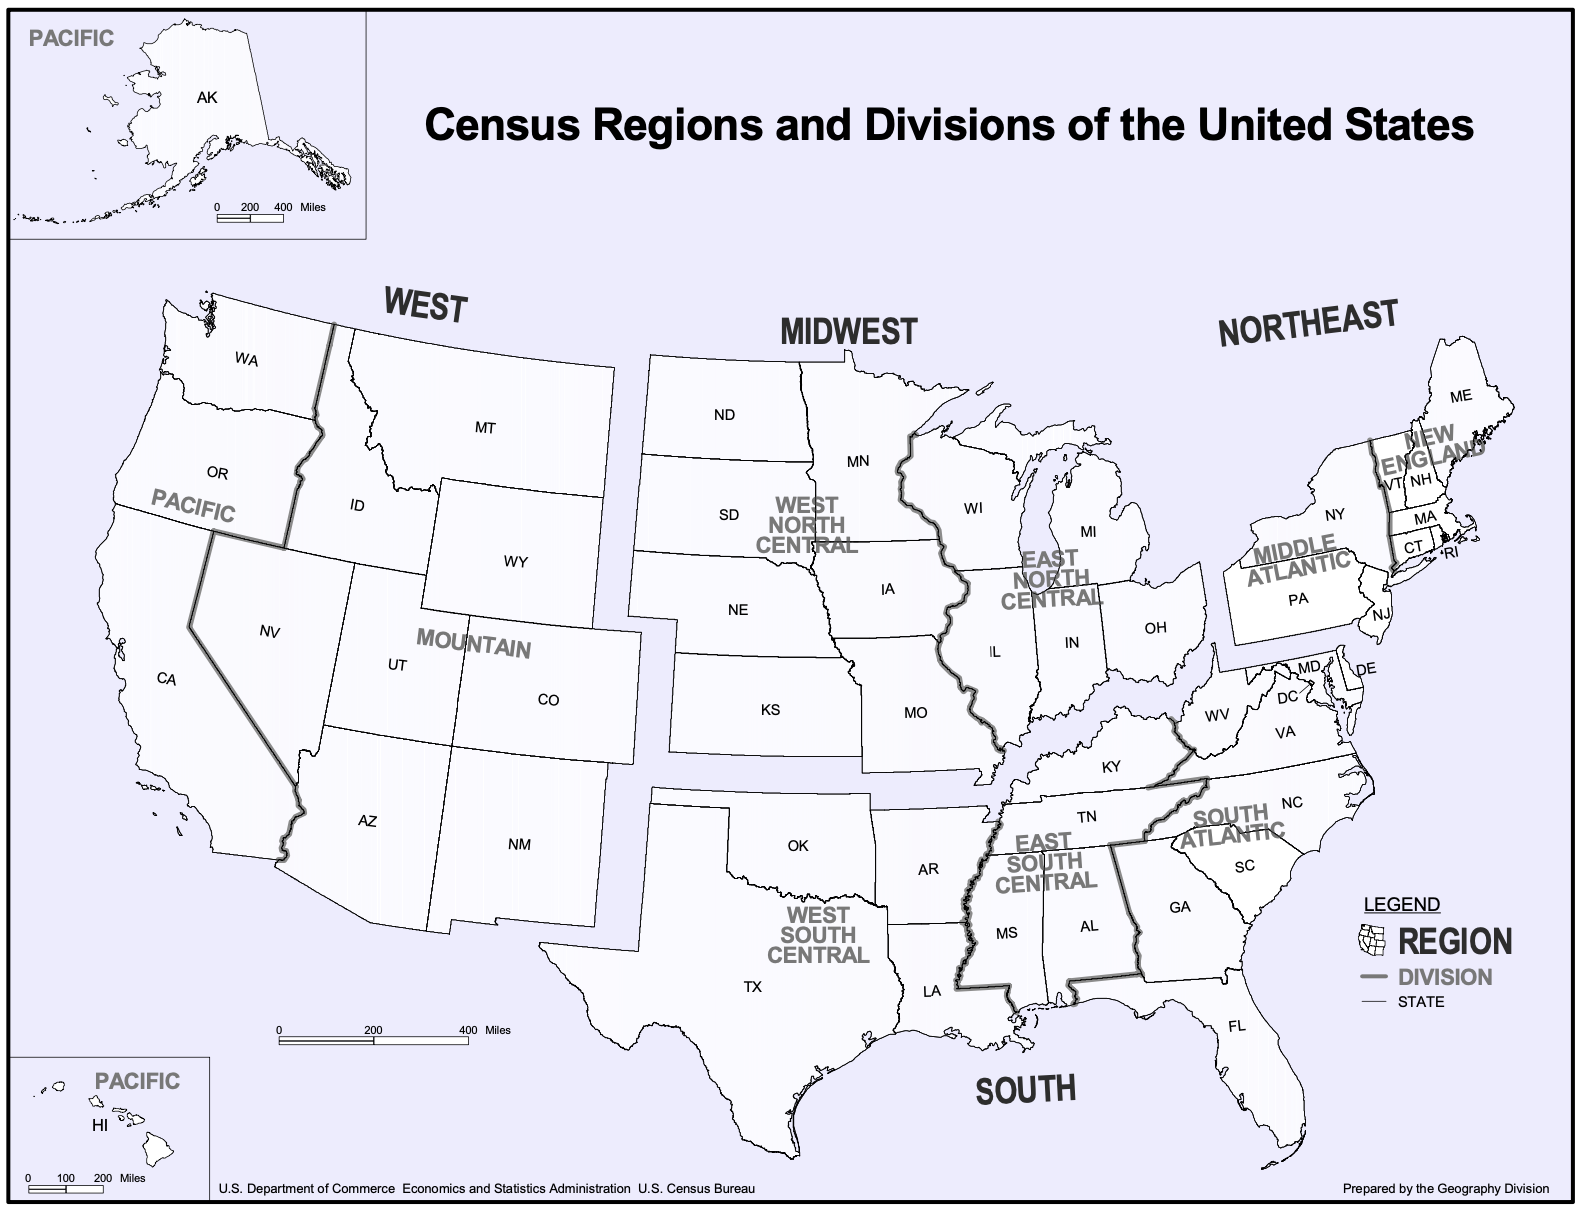
\includegraphics[width =\linewidth]{figures/us_region_map.png}
	
	\caption{Map showing geographical regions of the United States from the U.S. Census Bureau \parencite{regions}}
	\label{regionmap}
\end{figure}



% Our process in choosing which variables to choose then was matter of both process of elimination as well as positive testing. This process essentially worked in two ways, first we tried to determine the relationship between voting outcomes and a particular factors based on political science research. From the remain vaiables we then looked at different testing strategies for which covariates produced highly accurate prediction results.
\FloatBarrier
\subsection*{Data Cleaning}

We then merged these four datasets to created our own curated dataset. We did this by merging the different datasets on shared variables. As previously said, each observation represents a particular house district, so for the first three datasets, we simply merged them based on their state and district number. To include the regions we simply used the state variable for each district. 


In the election results dataset, we encountered one instance of missing data. For all of the districts in Louisiana, the winning party was not recorded. There was however the incumbant party recorded  in the Election Results dataset and by cross referencing this with public record we found for the 2022 House Election only candidates from the incumbant party remained in each of the districts. Therefore as is reflected in our code base we used the data from the incumbant party in place of winning party for the state of Louisiana. For all other states and disticts we did not encounter this problem. 

In terms of scaling we wanted all the variables to be on roughly the same scale to aid in convergence times. In order to do that we roughly scaled median income and total population by dividing total population by one million and dividing median income by one hundred thousand. This brought each of these to roughly the same scale as the other variables. Similarly we decided to scale all of the percentage variables to be on the scale zero to one hundred rather than zero to one to make their coefficents more interpretable.  

% \subsection{Covariate Choice}

% In addition to our main variable of interest, \textit{urbanindex} we had many covariates to choose from, not all of which ended up being used in our final models. There were also many more covariates that were present in our three datasets, however we decided to drop many of them as they were not relevant to our analysis. To create our initial list of covariates, we choose variables that we thought would capture education, income, or demographic make-up  of the districts because we thought they might be influential in determining partisan voting outcomes. How we choose our final covariates was a combination of domain knowledge and initial testing. Our intial list of covariates included:

% As previously explained, the districts are drawn in such a way that the total population of each district should be approximately the same \blue{cite}, so while this does help support our exchangability assumption, we determined that total population itself would be an unsuitable covariate. 


% To then build some knowledge into our models, we looked into different qualitative studies about voting behavior, which helped guide our final choices of covariates. 

\section{Code}


%Old 

%choices
%\begin{enumerate}
%	\item number of chains and iterations
%	\item brms i guess
%\end{enumerate}


%As our project consists of fitting a series of Bayesian multilevel linear models, we were able to do all of our modeling using the R package \verb|brms| \red{cite}.


%We fit each model with the function \verb|brm()|, with the usual R formula syntax, writing hierarchical effects with the random effects syntax (for eg, \texttt{Winning.party ~ urbanindex + (0 + urbanindex | Region ) + pct.retirees}). We add \verb|0| to the random effect because we are not interested in modeling a varying intercept.
%The priors are set according to what was laid out in Table \ref{tab:priors}.
%We chose to run 4 chains, with 4000 iterations each ... \red{Murthy please explain}%


% Leonor -


\red{MURTHY'S SECTION BEGINS}
%%%Copy this part
\blue{Here we should include a short description of every file that will be in report code that will be turned in with the report for example...}
To fit Bayesian Multilevel Models, one needs to use a probabilistic programming language.We used the R package \verb|brms| \parencite{brms}, which allows the user to code entirely in R while running STAN as the backend. In our zip folder there are \red{X number} R files. The file \textit{data\_cleaning.R} showing our process for combining our datasets.

The file \textit{modeling.R} contains the \verb|brms| code setting the priors and fitting our four models using the dataset obtained in \textit{data\_cleaning.R}.
The BRMS package allowed us to efficiently fit many models, as we needed only has to specify the model in a one- or two-line R formula. Each model was then fit with the function \verb|brm()|, using the usual R formula syntax. 
The priors are set according to what was laid out in Table \ref{tab:priors}.
For the parameter estimates we chose to run 4 chains with 4000 iterations each. We choose to run double the default number of iterations to get more information related to from the trace plots. Further, we set \texttt{save\_pars = save\_pars(all = TRUE)}, so that all parameter draws are saved. This was done to later perform moment matching when computing the LOO-CV statistics for model comparison, although it had no effect on the model estimates.

The file \textit{model\_comparison.R} is where we compute and plot the model comparison metrics described in Section \ref{sec:comparison}. The RMSE and LPD are obtained with the method described in \cite{brmsbook} \red{cite brms book, posterior model comparison}, and the LOO cross-validation is performed using the \verb|loo()| and \verb|loo_compare()|, also from the \verb|brms| package.

\red{INSERT PRIOR FILE NAME PLEASE} contains the code used to run the prior sensitivity analysis, using the alternative priors described in the corresponding section.

The file \textit{tables\_plots.R} contains code for generating tables used in the report (dataset descriptives, model estimates) as well as the marginal effects plots. Which were obtained with the \verb|conditional_effects()| function (setting the option \texttt{re\_formula = NULL}, to identify the group-level effects).


\blue{I think this bit belongs in the prior section to be honest*}
In brms the hierarchical coefficients are modelled as a centred Normal with a varying standard deviation, which itself follows a prior distribution given by the user \parencite{brmsbook}. \blue{*} 

%%%

% As our project consists of fitting a series of Bayesian multilevel linear models, we were able to do all of our modeling using the R package \verb|brms| \red{cite}.


% writing hierarchical effects with the random effects syntax (for eg, \texttt{Winning.party ~ urbanindex + (0 + urbanindex | Region ) + pct.retirees}). We add \verb|0| to the random effect because we are not interested in modeling a varying intercept. dont need this, or to explain this 



%Before running each model, we set the same seed (\verb|set.seed(1234)|) for reproducibility and to ensure that the differences between model results are due only to different prior/model specifications, not random differences in the sampling path. 

%\red{idk how much we're supposed to say here}



% Furthermore, we set \texttt{save\_pars = save\_pars(all = TRUE)}, so that draws from all variables defined in Stan's parameters block are saved. This has no effect on the model itself, and is only relevant in our case because we afterwards perform moment matching in computing the LOO-CV statistics for model comparison.

% \red{idk how much we're supposed to say here}



\section{Models}

%To describe our approach we wanted to test different models that incorporate the geographical hierarchy into the model. We made several common assumptions for the the four models that we compared with addtional more specific assumptions for each model. The first common assumption we made was that district voting outcomes can be modeled via logistic regression. This assumption gets at the basic logic of our models. As we said previously the outcomes of any particular district electoral race is binary (democrat/republic) so it is most appropriate to choose a modeling technique that can model binary outcomes. 
%
%\textit{Why did we choose logisitic regression?}
%
%We then moved on to our assumptions about the parameters of the linear regression model within the logistic regression model. We also assume that geography is a characteristic of each district that can be modeled hierarchical. For that reason we assume that each district is exchangeable within each state and that each state is exchangeable within each region. We assume this because for complicated historical reasons certain regiions of the united states are more similar to eachother than others. For example the Southern United states tends to be more religious and religous people tend to vote more conservatively, as a result the parameter associated with region would likely be smaller or more negative as compared to other regions. 
%We also are assuming that in some regions the value of urban index is more informative than others, the logic being that a city in a rural area will likely have stronger signal than an city among a bunch of other cities. 
%
%We also 
%
%++++++++++++++++++++++++++++++++++++++++++++

The \textit{Winning Party} in each congressional district race ($y_{i,j,k}$ for district $i$, state $j$, region $k$) can be modeled as the outcome of Bernoulli trial, since this is a binary variable: 
\begin{equation}
	y_{i,j,k} \sim Ber \left( \pi_{j,k} = logit^{-1}(\theta_{j,k})  \right)
\end{equation}
with probability of a Democrat win $\pi_{j,k}$ modeled as the inverse logit transform of $\theta_{j,k}$, a linear combination of our covariates. The inverse logit function converts real numbers into quantities between 0 and 1, and is therefore a standard way to model probabilities \parencite{logitlink}.


We tested four different models for $\theta_{j,k}$, which include different covariates in addition to our variable of interest (Urban index) and incorporate our data's hierarchical structure in different ways. Therefore, all four are Multilevel Bayesian (Logistic) Models, which require particular assumptions (\cite{BDA}): 
first, that a logistic regression accurately represents the relationship between the log-odds of a Democrat win and the explanatory variables, that is, $\theta_{j,k}$ and our covariates are linearly related; second, exchangeability, meaning that each district is exchangeable within each state and each state is exchangeable within each region; and third, that the value of urban index (and other covariates) in a district has a different effect depending on the state/region it belongs to.


The logistic relationship is common choice for modeling binary outcomes. It allows us to model the probability of a Democrat win by a linear predictor which can take any real value, while still having an interpretation for the coefficient estimates (in terms of change of log-odds).(\textcolor{red}{cite}).


We assume exchangeability because we assume that the districts are drawn in such a way that they are competitive for both parties. Meaning that although the districts may have different characteristics, certain mechanisms can be best captured when thinking of districts as exchangeable parts of  a hierarchical model. 
As an example, for complicated historical reasons, in certain regions of the United States Districts and States are more similar to each other to others outside of the region. For example, the South of the United states tends to be more religious, and religious people tend to vote more conservatively. We can think about this then as a prior telling us about the mix of democratic and republican districts within a particular state. Although the religiousity may increase the number of potential republican districts in each state, whether one district votes repuclican does not influence the decision of another since each district outcome is determined by thousands of individual votes. 

Since each district is part of a state and a region, we can translate the complex geographically determined mechanisms into our model by modeling some of parameters hierarchically.



We chose, however, not to include a varying Intercept in the linear predictor in any of our models. While the varying intercept could potentially improve the accuracy of our predictions, this is not our goal. We are interested primarily in the effect of urbanization on the election outcome in each district and how this effect can be modeled hierarchically. Therefore, we were more concerned with including other covariates in the linear predictor which could interfere with the estimated effect of Urban Index, and opted by leaving the random intercept out to keep the number of parameters to be estimated to a minimum.

% as a result the parameter associated with region would likely be smaller or more negative as compared to other regions. However the conditions for any particular southern state are the same, and 
% The idea behind the differing effect strength of urban index values per region is that a city in a rural area will likely have stronger signal than an city among a bunch of other cities. \textcolor{red}{[rewrite some of this paragraph]}



%\subsubsection*{Model 1}
%
%Model 1 is our most extensive model.
%
%Here we used urban index and 4 additional covariates plus an intercept to explain $\theta_{j,k}$.
%
%Both the state and region hierarchies were included, but on different covariates. Urban index and median income effects vary by state, while the slope of percentage of bachelor's degrees varies by region. The intercept and the slopes of percentage of women and percentage of retirees were considered to have the same effect for all districts, hence were modeled non-hierarchically.
%
%
%
%\begin{equation} \label{eq:big_uncentered}
%	\begin{aligned}
%		\theta_{j,k} = & \beta_0 + \beta_{women} \cdot \text{Pct\_Women} + \beta_{uncent \: urbindex, j} \cdot \text{Urban\_Index} \\
%		               & + \beta_{uncent \: bsc,k} \cdot \text{Pct\_Bach.} \\
%		               & + \beta_{uncent \: inc,j} \cdot \text{Median\_Income} + \beta_{ret} \cdot \text{Pct\_Retirees}
%	\end{aligned}
%\end{equation}
%
%
%
%Equation \ref{eq:big_uncentered} describes our model conceptually. In order to have a specification more compatible with R syntax so we can fit our model with brms, we reformulate the model as Equation \ref{eq:big_centered}, with the group-level (state or region) centered around zero, following \textcolor{red}{cite brms book}
%
%To better understand what happens in the backend when we want to fit this model with BRMS, it is helpful to rewrite the equation \ref{eq:big_uncentered} in terms of 'global' and 'hierarchical' effects.
%
%
%
%
%
%\begin{equation} \label{eq:big_centered}
%	\begin{aligned}
%		\theta_{j,k} = & \beta_0 + \beta_{women} \cdot \text{Pct\_Women}                                                                              \\
%		               & + \beta_{urbindex} \cdot \text{Urban\_Index} + \beta_{urbindex, j} \cdot \text{Urban\_Index}                                 \\
%		               & + \beta_{bsc} \cdot \text{Pct\_Bachelor's} + \beta_{bsc,k} \cdot \text{Pct\_Bach.} + \beta_{inc} \cdot \text{Median\_Income} \\
%		               & + \beta_{inc,k} \cdot \text{Median\_Income} + \beta_{ret} \cdot \text{Pct\_Retirees}
%	\end{aligned}
%\end{equation}
%
%Note that although we are interested in hierarchically varying coefficients for certain variables, we nevertheless include a non-varying coefficient for the same variables, e.g. we have both a global coefficient as well as a state dependent coefficient for urban index. 

%\subsubsection*{Model 2} 
%
%For Model 2 we significantly reduced the number of variables. We kept only our variable of interest, urban index, and percentage of retirees \textcolor{red}{[why?????]}
%Here, the geographical hierarchy was incorporated through a \textit{nested hierarchy} of districts within states within regions.
%So, this model assumes that the effect of urbanindex ($\beta_{urb, j:k}$) depends on state $j$ and region $k$ through a prior with mean parameter $\beta_{urb, k}$, which in turn varies by region and depends on hyper-mean $\beta_{urb}$ (which has its own prior, with hyper-hyper-parameters). Equation \ref{eq:nested_centered} specifies the model, with the centered around zero formulation. 
%% Model equation
%\begin{equation} \label{eq:nested_centered}
%	\begin{aligned}
%		\theta_{j,k} =    &\beta_0 + \beta_{urb} \cdot \text{Urban\_Index} + \beta_{urb,k} \cdot \text{Urban\_Index} \\
%		&+ \beta_{urb,j:k} \cdot \text{Urban\_Index} + \beta_{ret} \cdot \text{Pct\_Retirees}
%	\end{aligned}
%\end{equation}





%
%
%\subsubsection*{Model 3}
%
%
%
%
%\begin{equation} \label{eq:state_level_centered}
%	\begin{aligned}
%		\theta_{j} =    &\beta_0 + \beta_{urb} \cdot \text{Urban\_Index} + \beta_{urb,j} \cdot \text{Urban\_Index} \\
%		&+ \beta_{ret} \cdot \text{Pct\_Retirees}
%	\end{aligned}
%\end{equation}





%\subsubsection*{Model 4}
%
%
%
%
%\begin{equation} \label{eq:region_level_centered}
%	\begin{aligned}
%		\theta_{k} =    &\beta_0 + \beta_{urb} \cdot \text{Urban\_Index} + \beta_{urb,k} \cdot \text{Urban\_Index} \\
%		&+ \beta_{ret} \cdot \text{Pct\_Retirees}
%	\end{aligned}
%\end{equation}






\subsubsection*{Model 1 (state level)}


Our first model includes only our variable of interest, urban index, plus the percentage of retirees as covariates to explain $\theta$, plus an intercept.
\blue{ Murthy didn't you find something in initial testing? please write about that.
M: In the very initial fits with all default settings and no hierarchies, percentage retirees consistently had less convergence issues. But I don't want to write new code for this now...plus we've made a lot of changes since the initial stage, idk how things will behave now. Maybe I can come up with a logical rather than technical reason??}
\red{it has the strongest correlation with winning party after urban index, and it's the only one negatively correlated with winner, could we justify it one of those ways?}

Urban index was modeled hierarchically, with the coefficient varying by state, with a prior dependent on common parameters $\beta_{urb}$ and $\sigma_{urb}$, which in turn have (hyper-)priors of their own. The intercept is assumed to be non-variant for all districts, as well as the slope of percentage of retirees.

Equation \ref{eq:state_level_uncentered} describes our model conceptually.


\begin{equation} \label{eq:state_level_uncentered}
	\begin{aligned}
		\theta_{j} =    &\beta_0 + \beta_{urb,j}^{uncent} \cdot \text{Urban\_Index} + \beta_{ret} \cdot \text{Pct\_Retirees}
	\end{aligned}
\end{equation}

To better understand what happens in the backend when we want to fit this model with BRMS, it is helpful to rewrite the equation \ref{eq:state_level_centered} in terms of 'global' and 'hierarchical' effects. The previously considered coefficient is then decomposed into these effects, i.e.
$\beta_{urb,j}^{uncent} = \beta_{urb} + \beta_{urb,j}$
with $\beta_{urb,j}$ centered around zero, which does not alter the meaning of the model (\cite{brmsbook}).

\begin{equation} \label{eq:state_level_centered}
	\begin{aligned}
		\theta_{j} =    &\beta_0 + \beta_{urb} \cdot \text{Urban\_Index} + \beta_{urb,j} \cdot \text{Urban\_Index} \\
		&+ \beta_{ret} \cdot \text{Pct\_Retirees}
	\end{aligned}
\end{equation}


Although we assume that there is indeed state-level clustering in the district election outcomes, we have 50 states, and some of them include only one or two districts. This can make the hierarchical estimates unreliable. 


\subsubsection*{Model 2 (region level)}


To overcome this problem, we fit another model, with only one difference from the previous one: the hierarchy is at the region level, rather than state. This means the coefficients of urban index vary by region now, with a common mean and variance which are parameters to be estimated themselves.
Equation \ref{eq:region_level_centered} describes this model, in its specification with separate global and hierarchical effects for urban index.


\begin{equation} \label{eq:region_level_centered}
	\begin{aligned}
		\theta_{k} =    &\beta_0 + \beta_{urb} \cdot \text{Urban\_Index} + \beta_{urb,k} \cdot \text{Urban\_Index} \\
		&+ \beta_{ret} \cdot \text{Pct\_Retirees}
	\end{aligned}
\end{equation}

%The theoretical reasoning for this model is not as strong. 

\subsubsection*{Model 3 (nested)}


In this model we include the entire geographical hierarchy: a \textit{nested hierarchy} of districts within states within regions.
Here the assumption is that the effect of urbanindex ($\beta_{urb, j:k}$) depends on state $j$ and region $k$ through a prior with mean parameter $\beta_{urb, k}$, which in turn varies by region and depends on hyper-mean $\beta_{urb}$ (which has its own prior, with hyper-hyper-parameters). Equation \ref{eq:nested_centered} specifies the model, with the centered around zero formulation. 

% Model equation
\begin{equation} \label{eq:nested_centered}
	\begin{aligned}
		\theta_{j,k} =    &\beta_0 + \beta_{urb} \cdot \text{Urban\_Index} + \beta_{urb,k} \cdot \text{Urban\_Index} \\
		&+ \beta_{urb,j:k} \cdot \text{Urban\_Index} + \beta_{ret} \cdot \text{Pct\_Retirees}
	\end{aligned}
\end{equation}



\subsubsection*{Model 4 (big model)}


This is our most extensive model.
Here we used urban index and 4 additional covariates plus an intercept to explain $\theta_{j,k}$.
It can be seen as an extension of Model 1, as urban index is modeled hierarchically by state. The region level hierarchy is instead included only in the effect of percentage of bachelors degrees.
Median income effect is also considered to vary by state, and the intercept and the slopes of percentage of women and percentage of retirees were modeled non-hierarchically.

Equation \ref{eq:big_centered} describes this model, in the brms adapted specification.

\begin{equation} \label{eq:big_centered}
	\begin{aligned}
		\theta_{j,k} = & \beta_0 + \beta_{women} \cdot \text{Pct\_Women}                                                                              \\
		& + \beta_{urbindex} \cdot \text{Urban\_Index} + \beta_{urbindex, j} \cdot \text{Urban\_Index}                                 \\
		& + \beta_{bsc} \cdot \text{Pct\_Bachelor's} + \beta_{bsc,k} \cdot \text{Pct\_Bach.} + \beta_{inc} \cdot \text{Median\_Income} \\
		& + \beta_{inc,k} \cdot \text{Median\_Income} + \beta_{ret} \cdot \text{Pct\_Retirees}
	\end{aligned}
\end{equation}













\section{Priors} \label{sec:priors}

Priors represent our initial beliefs about our model parameters' distributions.
In each of our models, this means a prior for the intercept, one for the slope of each covariate that is modeled non-hierarchically (e.g., $\beta_{ret}$ in all four models) and, in the case of covariates with global and hierarchical effects, priors for the hyper-parameters as well.

Table \ref{tab:priors} lists our selected priors for each model, by corresponding covariate.

\begin{table}[h]
	\resizebox{\textwidth}{!}{%
		\begin{tabular}{l|llll}
			\toprule
			              & \multicolumn{1}{c}{Model 1}              & \multicolumn{1}{c}{Model 2}              & \multicolumn{1}{c}{Model 3}                  & \multicolumn{1}{c}{Model 4}                  \\ \hline
			Intercept     & $\beta_0 \sim N(0, 10)$                  & $\beta_0 \sim N(0, 10)$                  & $\beta_0 \sim N(0, 10)$                      & $\beta_0 \sim N(0, 10)$                      \\
			Urban Index   & $\beta_{urb} \sim N(0,1)$                & $\beta_{urb} \sim N(0,1)$                & $\beta_{urb} \sim N(0,1)$                    & $\beta_{urb} \sim N(0,1)$                    \\
			              & $\beta_{urb, j} \sim N(0, \sigma_{urb}),$ & $\beta_{urb, k} \sim N(0, \sigma_{urb}), $ & $\beta_{urb, k} \sim N(0, \sigma_{urb,1}), $     & $\beta_{urb, j} \sim N(0, \sigma_{urb}), $ \\
			              & $\sigma_{urb} \sim Halfcauchy(10)$         & $\sigma_{urb} \sim Halfcauchy(10)$     & $\sigma_{urb,1} \sim Halfcauchy(10)$             & $\sigma_{urb} \sim Halfcauchy(10)$         \\
			              &                                          &                                          & $\beta_{urb, j:k} \sim N(0, \sigma_{urb,2}), $ &                                              \\
			              &                                          &                                          & $\sigma_{urb,2} \sim Halfcauchy(10)$           &                                              \\
			Pct.retirees  & $\beta_{ret} \sim t(1,-2,1)$             & $\beta_{ret} \sim t(1,-2,1)$             & $\beta_{ret} \sim t(1,-2,1)$                 & $\beta_{ret} \sim t(1,-2,1)$                 \\
			pct.women     &                                          &                                          &                                              & $\beta_{women} \sim N(0,1)$                  \\
			pct bsc       &                                          &                                          &                                              & $\beta_{bsc} \sim t(1,0,1)$                  \\
			              &                                          &                                          &                                              & $\beta_{bsc, k} \sim N(0, \sigma_{bsc}), $ \\
			              &                                          &                                          &                                              & $\sigma_{bsc} \sim Halfnormal(0,1)$        \\
			median income &                                          &                                          &                                              & $\beta_{inc} \sim N(0,1)$                    \\
			              &                                          &                                          &                                              & $\beta_{inc, j} \sim N(0, \sigma_{inc}), $ \\
			              &                                          &                                          &                                              & $\sigma_{inc} \sim Halfnormal(0,1)$        \\ \bottomrule
		\end{tabular}%
	}
	\caption{Priors defined for each of our four models, for each parameter; parameters and distributions are listed by their corresponding covariate.}
	\label{tab:priors}
\end{table}



We define such distributions before seeing the data, based on existing literature and our own intuition about the effects of our covariates on the probability of a democrat win.
We assumed the same priors for the same terms included in different models (intercept, percentage of retirees, urban index for the same levels).

%For many of our parameters we picked Normal distributions [reasons]

For the intercept $\beta_0$ we set a Normal prior centered at zero with a large standard deviation. 
This represents a weakly informative prior, as we had no strong beliefs about the intercept value, nor does it have any straightforward interpretation in our model.
%our assumption that the probability of either party winning is roughly 50\% (corresponding to a $\theta_{j,k}$ of zero) when all other factors are absent. [wrong]


%%%%%%%%%%%%%%%%%% urban index %%%%%%%%%%%%%%%%%%%%%%%%
For the population-level component of the \textit{Urban Index} slope we opted for a standard normal prior in all models. We chose not to make assumptions on the sign of the effect of this variable, as it is this variable that we are interested in studying, although we are assuming that its absolute value will be below 1.96 with 95\% certainty. 
%So, we set comparatively less-informative priors on the parameters representing the effect of the index.

All group-level (zero-centered) priors are Normal, by \verb|brms| specification \textcolor{red}{is there a reason??? M: Yes, but we'll have to dig deep into the MC Stan Forums and see what Paul wrote. Explaining this is out of the scope tbh. Refer to one of my paras where I mention BRMS is simply less flexible than STAN, I could add a couple lines there}\blue{yes please add those sentences}
\red{we can just keep the black here, this was added to the limitations already}

For the standard deviation of the hierarchical effects we opted for a relatively weakly informative prior, a $(half)Cauchy(0,10)$.
We do not want to place strong constraints on the effect of our variable of interest, hence we 'allow the estimates to fluctuate'.



%%%%%%%%%%%%%%%%%%% pct_ret %%%%%%%%%%%%%%%%%%%%%%%
As found in the literature older voters tend to vote more conservatively \parencite{brown2022oldvoters}, so it makes sense that a higher the \textit{Percentage Retirees} in each district negatively correlates with the probability of a Democrat winning, but we do not know how strong this effect ought to be. Therefore, for the prior on $\beta_{ret}$ we chose a distribution centered around a negative number, and with relatively heavy tails, reflecting our uncertainty, for all models. 



%%%%%%%%%%%%%%%%%%%%%%%% women %%%%%%%%%%%%%%%%%%%%
In Model 4, \textit{Percentage Women} is not modeled hierarchically.
Although women tend to vote more democratic and have higher voter turnout \parencite{pew2020}, the percentage of women is roughly the same in every district, so we do not expect this covariate to have a strong effect on the probability of either party winning, i.e, we expect $\beta_{women}$ to be close to zero. So, we set a prior for this slope which is centered around zero and has little variability: a standard normal prior. 



The effects of \textit{Percentage of Bachelors} degrees and \textit{Median Household Income} are parameterized in 2 hierarchical levels: an average slope across all districts, and a varying slope by group (State or Region), $\beta_{covariate,j}$ or $\beta_{covariate,k}$, which follows a Normal distribution centered at zero with standard deviation modeled at group level (by a hyperprior). This was done to capture the idea of different costs of living and importance of education respectively, as what is considered rich, poor, or well educated for an individual is highly dependent on the environment. 
%\red{what do u think?}

 

As we expected the population-level effects of both \textit{Median Houshold Income} and \textit{Percentage Bachelors} to be positive in some cases and negative in others, we picked symmetric priors for both $\beta_{bsc}$ and $\beta_{inc}$. We are, however, less sure about the on-average-null effect of the \textit{Percentage of Bachelor} degrees, so for this slope parameter we opted for a prior with 'fatter tails', the standard Cauchy distribution rather than the Normal one, representing a higher degree of uncertainty.


For the hyperparameters, we chose a half standard normal prior for both the standard deviations of $\beta_{bsc,k}$ and $\beta_{inc,j}$. This is a narrow distribution, with most values falling between 0 and 1, as we expect to see weak effects for these covariates, and thus small standard deviations (and positive, as any SD is by definition).











\section{Results}

%\textcolor{red}{This section is not on the instructions but is probably the easiest way to talk about the results we got }


Each of our models has different estimates for the parameters, even when they are starting from the same prior.
As the estimate is given by the mean of the posterior distribution for that parameter, this reflects the different posterior distributions between models, which is only natural given the different structures each model assumes for our data.

The intercept for example, is very different between models, and is particularly large (in absolute terms) in Model 4. Although, as discussed before, the intercept does not have a practical interpretation in our model, it is interesting that this Model's estimate is so far away from the value we initially assumed it would take (between -19.6 and 19.6 with 95\% certainty, with a $N(0,10)$ prior).

Our variable of interest, \textit{Urban Index}, has a more consistent slope estimate across models, between 1.22 (Model 2) and 1.66 (Model 1).
Figure \ref{fig:urbanindex_estimates} shows the histograms of posterior draw for the \textit{Urban Index} slope parameter, by Model.
The results indicate that the variable has, as expected, on average a positive effect on the log-odds of a Democrat Party win.
Model 3, for example, estimates that on average a 1 unit increase in \textit{Urban Index} (e.g., 10 to 11) translates into a 1.64 increase in the log-odds (or an $e^{1.64} \approx 5.155 $ increase in the odds) of a Democrat being elected in the district.
While the estimates are within the range we assumed with the prior for this parameter, the upper bounds of the credible intervals are already close to the boundary of that prior. 
%The data has updated our beliefs about the effect of this variable a lot.
A prior with more probability mass on the positive range, or a less informative prior, could push the estimates further up.

\begin{figure}
	\centering
	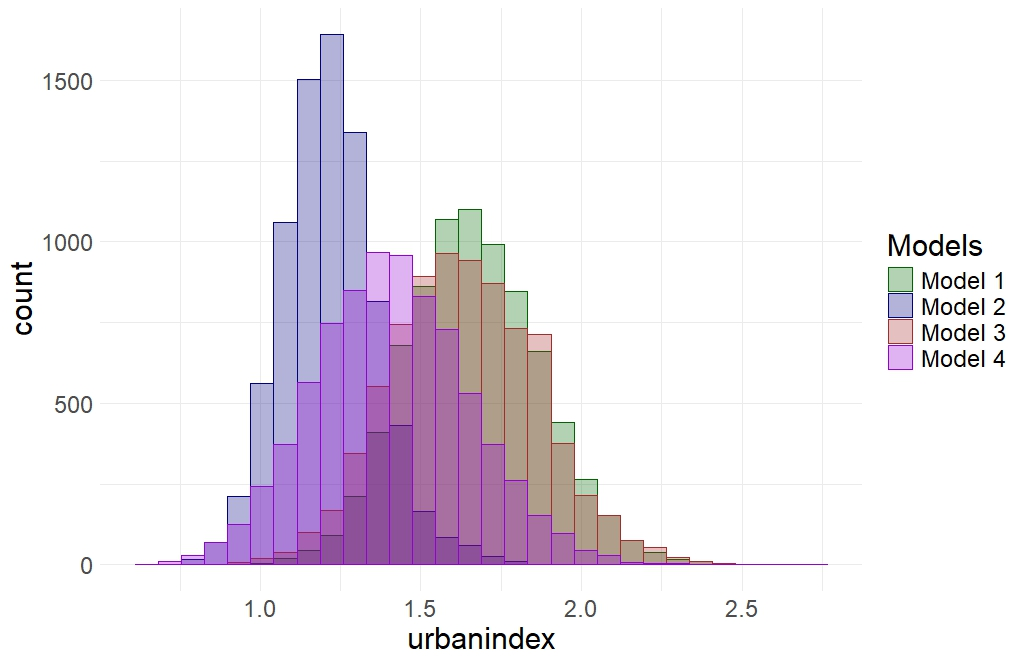
\includegraphics[width=0.7\textwidth]{results/urb_post_all_models.jpeg}
	\caption{Histogram of posterior draws of Urban Index effect, all models}
	\label{fig:urbanindex_estimates}
\end{figure}

The standard deviation estimates for the hierarchical effect of \textit{Urban Index}  are all on the lower side of the prior, close to zero. This is true both for the cases when the hierarchy on \textit{Urban Index} includes \textit{State} or \textit{Region}.


The estimated slope of \textit{Percentage Retirees} is also different between models, particularly in Model 4, where it is larger in absolute value, but always negative as we had assumed. Note that although this estimate is smaller in absolute terms than the slope of \textit{Urban Index}, it does not mean that \textit{Percentage of Retirees} has a weaker effect than urbanization in election outcome. These are different variables on a different scale: in model 3 for example, it is estimated that an increase of 1 percentage point in the percentage of retirees in a district correlates with a 0.16 decrease in the log-odds of a Democrat being elected.

The other covariates included in model 4 also have slope estimates within our expected range.
Median Income has a larger (absolute) estimated slope coefficient and standard deviation, but this is likely due to the scale of the variable: 1.43 is the estimated average decrease in log-odds of a Democrat win when the median income of a district increases by 100,000 dollars, which is a big jump. The inclusion of these covariates has some effect on the magnitude of the slope estimate for our variable of interest (\textit{Urban Index}), but not on its sign, and not as much as including a State-specific hierarchical effect vs. Region-specific one.


%for the conditional effects all parameters not part of the condition you investigate are set to their mean/reference category.


While the estimated effect is not so different between models, the credible intervals are another story. Figure \ref{fig:cond_effects} shows the plotted estimated marginal effect of \textit{Urban Index} on the probability of a Democrat winning according to models 1 and 2, accounting for group-level effects. Model 1 estimates much wider credible intervals than 2. This is due to the number of levels in each model: more levels result in higher uncertainty.
and (possibly) to the fact that in model 1 there are several levels with a very small number of observations.

\begin{figure}[h] 
	\centering
	\begin{subfigure}{0.45\textwidth}
		\centering
		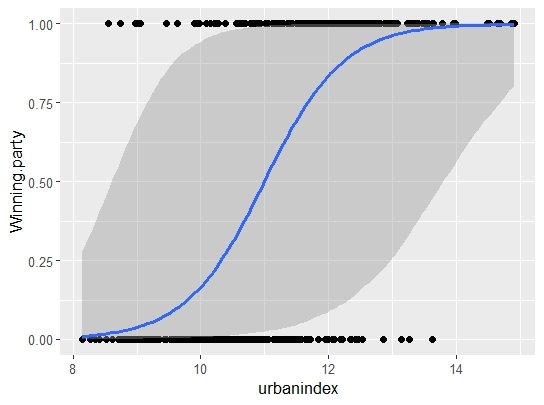
\includegraphics[width=\linewidth]{results/cond_eff_urb_model1_groupeff.jpeg}
		\subcaption{Model 1}
		\label{fig:subfig1}
	\end{subfigure}
	\hfill
	\begin{subfigure}{0.45\textwidth}
		\centering
		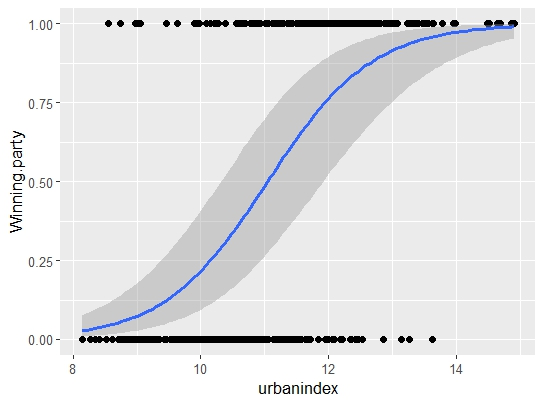
\includegraphics[width=\linewidth]{results/cond_eff_urb_model2_groupeff.jpeg}
		\subcaption{Model 2}
		\label{fig:subfig2}
	\end{subfigure}
	\caption{Conditional effects of \textit{Urban Index}, for Models 1 and 2; mean in blue, with 95\% credible intervals in gray, observations in black;  group level effects included}
	\label{fig:cond_effects}
\end{figure}



\FloatBarrier
\section{Convergence Diagnostics}

One of the fundamentals of Bayesian analysis is its reliance on MCMC sampling. This ensures we have access to both the posterior samples and the estimates of the posterior regression coefficients. All our data analysis was done using BRMS, which runs on STAN, which itself uses the Hamiltonian Monte Carlo algorithm for the posterior generation. 

\blue{*}"Convergence " in layman's terms can be described as, 'Do the posterior draws get closer and closer to a specific value?'. \blue{ * considering audience I don't think we need this sentence}

HMC Convergence diagnostics can be a rather extensive topic, so for this project we mainly consider graphical diagnostics, namely: the MCMC trace plots as provided by the \texttt{brms} package.

\begin{figure}
	\centering
	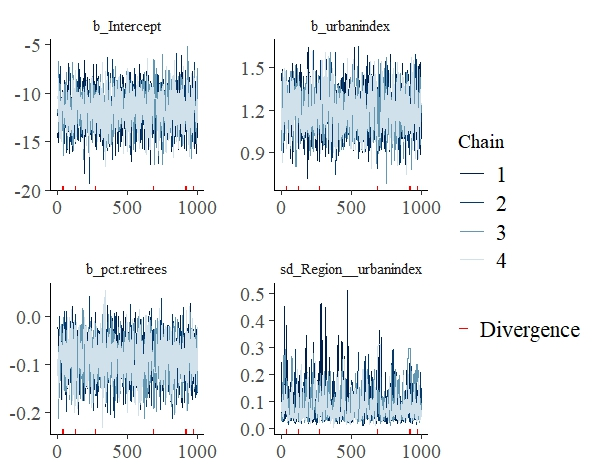
\includegraphics[width=0.7\textwidth]{trace_plots/trace_model2.jpeg}
	\caption{Trace plots for Model 2, all parameters; 2000 sampling iterations}
	\label{fig:trace_mod2}
\end{figure}

%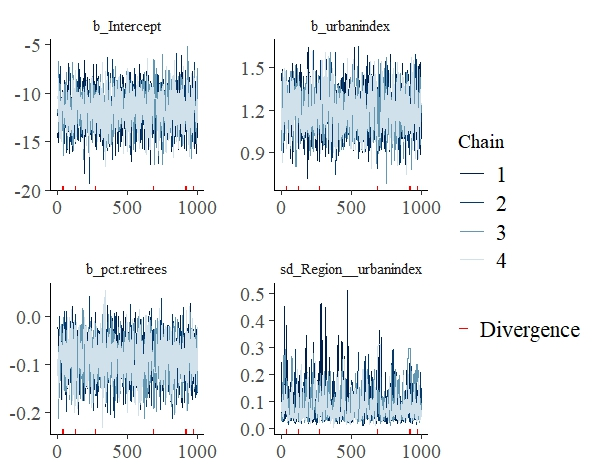
\includegraphics[scale = 1.2]{trace_plots/trace_model2.jpeg}

\begin{figure}
	\centering
	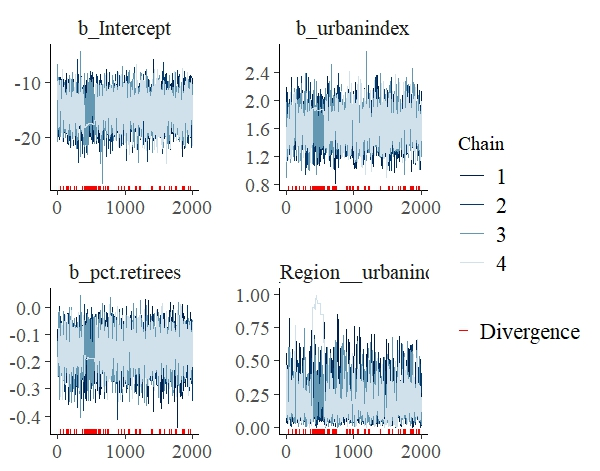
\includegraphics[width=0.7\textwidth]{trace_plots/trace_model3_part1.jpeg}
	\caption{Trace plots for Model 3, intercept, slopes and SD for Region level; SD for the lower level (Region:State) in Appendix; 2000 sampling iterations}
	\label{fig:trace_mod3_p1}
\end{figure}

%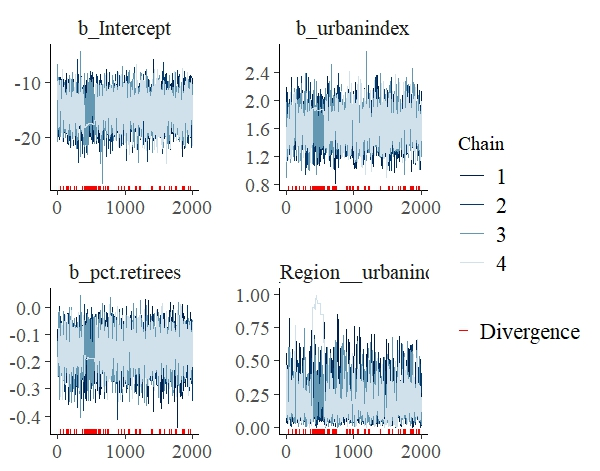
\includegraphics[scale = 1.2]{trace_plots/trace_model3_part1.jpeg}

We present the trace plots for Model 2 (Fig. \ref{fig:trace_mod2}) and most coefficients of Model 3 (Fig. \ref{fig:trace_mod3_p1}). Although we see divergent transitions in both cases, there are two key differences:

Firstly, the number of divergent transitions: There are many more of these for Model 3 in comparison to Model 2. Secondly, the place of occurrence: Model 3's divergent transitions occur throughout the chains, while those in Model 2 seem to be concentrated around the 1000th iteration, while noticeably decreasing towards the 2000th iteration. This suggests that increasing iterations further might help with Model 2, but is unlikely to help with Model 3. \blue{when you say "might help with" what do you mean? Might help with what exactly? }

The trace plots of the other models and coefficients (in Appendix) either resemble those of Model 2 \blue{how so?}, or  have no divergent transitions as is the case with Model 1.

Our key takeaway is the HMC chains behave strangely  \blue{when you say behave strangely what does that mean? try to be specific} for Model 3, and reasonably for the rest provided we increase the number of iterations from the default 1000 to 2000. \red{Luckily for us, there is one glaring difference between Model 3 and the rest which partially explains this behaviour: Namely,} \blue{this is really informal, you could also just write: "This is likely due to Model 3 being .."} it is the only model which takes into account both a Region-wise hierarchy and a State-wise hierarchy for the same coefficient, with the former being nested in the latter. The other models have at most a single hierarchy per coefficient. 

While this in itself is not enough to conclude that the specifications of the other models are correct, it is certainly a good preliminary finding \blue{good preliminary finding of what?}(that the presence of an explicit nested hierarchy causes HMC chain convergence issues). 


\section{Model Comparison} \label{sec:comparison}


Our four models were built based on somewhat different assumptions about the structure of our data, and all produced slightly different results. To better answer our research question, we need to know which of these is \textit{better} prediction-wise.
%, that is, which results are more trustworthy and allow us to answer our original research question.
To this end, we measured and compared our models' predictive performance using different metrics. %first by looking at absolute in-sample predictive performance, then at relative and finally at the Leave-One-Out statistics to compare out-of-sample Predictive Performance.


Absolute predictive performance metrics directly tell us how well the model performs, without looking at other models.
To measure absolute predictive performance we used the Root Mean of Squared Error (RMSE). The RMSE for the $s$-th posterior draw is obtained from the predictive errors, that is, observed outcome $y_n$ minus posterior draw $\hat{y}_n^{(s)}$, squaring those errors and taking the root of their average over all observations, i.e.,
$$
RMSE^{(s)} = \sqrt{
	\frac{1}{N} 
	\sum_{n = 1}^{N}
	\left( y_n - \hat{y}_n^{(s)} \right)^2
}
$$
Since it is computed for each draw, as opposed to a single point estimate, it takes into account the posterior uncertainty.
%making it a fully Bayesian measure \blue{citation needed?}.

%\begin{equation} \label{eq:rmse}
%	RMSE^{(s)} = \sqrt{
%		\frac{1}{N} 
%		\sum_{n = 1}^{N}
%		\left( y_n - \hat{y}_n^{(s)} \right)^2
%		}
%\end{equation}


%\blue{this section should go before the previous few paragraphs of the model comparison but after the equation explaination. from here **}
%The RMSE measure works in a similar way to the R squared statistic that is commonly used to assess the fit of linear models, by evaluating differences between observations and model predictions, but RMSE retains the scale of the response variable.
The RMSE retains the scale of the response variable.
Usually this would mean it has a direct interpretation in the context of the problem, but here we are dealing with a binary response variable, so what the RMSE actually represents is the average distance between the predicted value and 0 or 1, not the true probability of a Democrat win.
A model with higher RMSE in this context is not necessarily better at estimating this true value, just on average estimates probability values that are larger for districts where a Democrat won and smaller where a Republican won instead. 
%\blue{** to here }

%Figure \ref{fig:rmse} shows the histograms of the RMSE with all draws for each of our models.
Model 4, with higher RMSE, estimates on average closer percentages to the actual outcome which, in a certain sense, can mean it estimates voting outcomes better. This is unsurprising, as this model has many more covariates, and at least some have a large effect on the probability of a Democrat win.
%More important for our analysis is the comparison between models 1,2 and 3.
Model 2 has the largest average errors, which can mean this model's predictions are more often "wrong" (estimates small probability when a Democrat has won or large otherwise) or that the predictions are in general closer to the center (0.5) rather than the extremes. 
%In either case, it suggests that the Region-level hierarchy in urbanindex is not as powerful as the State-level one for estimating probabilities.
Model 3 has on slightly smaller RMSE values than Model 1, suggesting the inclusion of the Region hierarchy really does not have a large impact on posterior predictions.



%
%\blue{this section should go before the previous few paragraphs of the model comparison but after the equation explaination. from here **}
%The RMSE measure works in a similar way to the R squared statistic that is commonly used to assess the fit of linear models, by evaluating differences between observations and model predictions, but RMSE retains the scale of the response variable.
%Usually this would mean it has a direct interpretation in the context of the problem (e.g., by how many units is our prediction off), but here we are dealing with a binary response variable, so what the RMSE actually represents is the average distance between the predicted value and 0 or 1, not the true probability of a Democrat win.
%A model with higher RMSE in this context is not necessarily better at estimating this true value, just on average estimates probability values that are larger for districts where a Democrat won and smaller where a Republican won instead. 
%\blue{** to here }
%






Relative predictive performance measures, contrary to absolute ones, do not have an interpretation in themselves, only as a comparison between models. 
To assess relative predictive performance, we looked at log-likelihood scores, that is, the average of posterior draws' log-likelihoods for each observation.
This is a relative predictive performance measure in the sense that it does not tell us anything about the model's predictive performance alone, rather we need to compare it between different models to establish which is better. So, we examine the differences in log-likelihood scores between models.
The sum of these differences corresponds to the difference in Log Predictive Density (LPD) between models, where LPD for a given model is the sum of Log-Likelihood scores of all observations in the model.

%Figure \red{WILL BE HERE} shows the histograms of these differences for all 435 observations.



% latex table generated in R 4.3.2 by xtable 1.8-4 package
% Thu Mar  6 00:46:46 2025
\begin{table}[ht]
	\centering
	\begin{tabular}{lcc}
		\hline
		       Comparison & LPD\_Diff & SE\_LPD\_Diff \\ 
		       \midrule
		Model 1 - Model 2 &     42.00 &          7.25 \\
		Model 1 - Model 3 &     -2.32 &          1.29 \\
		Model 1 - Model 4 &    -20.24 &          3.91 \\
		Model 2 - Model 3 &    -44.32 &          7.31 \\
		Model 2 - Model 4 &    -62.24 &          8.20 \\
		Model 3 - Model 4 &    -17.92 &          3.66 \\ \hline
	\end{tabular}
	\caption{LPD differences between models, with respective standard errors}
	\label{tab:LPD_diff}
\end{table}

Table \ref{tab:LPD_diff} shows the differences in LPD between all four of our models and corresponding standard errors.
Model with higher LPD are preferred, as this reflects an overall higher (less negative) log-likelihood score across all observations, meaning the model more accurately predicted each result.
The difference between Models 1 and 2 is positive, meaning Model 1 has higher LPD, so it is preferred over 2 using this statistic. In fact, Model 2 is never preferred to any of the other models. Once again, Model 4 provides the best fit and Models 1 and 3 are very close, with 3 performing slightly better. This, together with the comparatively poorer fit of Model 2 points towards Region-level hierarchy possibly not being the correct choice for modeling \textit{Urban Index}.

%Note: these metrics are in-sample, so is biased towards more complex models 


Both RMSE and LL scores are in-sample predictive performance metrics. In-sample predictive performance measures evaluate only model predictions for the same observations which were used to fit the model in the first place, therefore they only evaluate how well a model predicts the data it was trained on, which means there is a danger of overfitted models, that would not generalize well to new data, performing much better under these metrics (\cite{brmsbook}).
%In our case, the bigger model (Model 4) was indeed the preferred one using both RMSE and LL scores.
It is essential to check also out-of-sample predictive performance metrics. These metrics are computed by splitting the dataset into training data and test data, fitting the model on the former and computing the expected LPD (ELPD) of the observations in the latter, given the model estimates with the training set. 

%\begin{equation}
%	ELPD = \sum_{n= 1}^{\tilde{N}} p(\hat{y}_n | y) 
%%	\approx
%%	\sum_{n= 1}^{\tilde{N}} \frac{1}{S} \sum_{s = 1}^{S}  log p(\tilde{y}_n | \theta^{(s)}) 
%\end{equation}
The way we choose to split the data into training/test sets naturally impacts the ELPD. So, we rely on cross-validation: we do multiple different splits and average over the results. Our chosen method was Leave-One-Out (LOO) cross-validation, which in theory performs as many splits as observations in the dataset, each time leaving one 'out' as the test data. In practice, a different posterior is not actually computed this many times, but rather an estimate from the full model posterior using importance sampling (Pareto-Smoothed Importance Sampling in this case).

\begin{table}[ht]
	\centering
	\begin{tabular}{rcccccccc}
		\hline
		& elpd\_diff & se\_diff & elpd\_loo & se\_elpd\_loo & p\_loo & se\_p\_loo & looic & se\_looic \\ 
		\hline
		Model 4 & 0.00 & 0.00 & -156.49 & 11.59 & 32.57 & 3.25 & 312.98 & 23.19 \\ 
		Model 3 & -17.99 & 4.23 & -174.48 & 12.11 & 33.08 & 3.33 & 348.97 & 24.22 \\ 
		Model 1 & -20.35 & 4.61 & -176.84 & 12.09 & 33.37 & 3.43 & 353.68 & 24.18 \\ 
		Model 2 & -45.87 & 8.39 & -202.36 & 12.25 & 6.19 & 0.58 & 404.71 & 24.50 \\ 
		\hline
	\end{tabular}
	\caption{LOO statistics for all models}
	\label{tab:loo}
\end{table}

According to the LOO statistics (Table \ref{tab:loo}), Model 4 (the largest) is the preferred one, followed by Models 3, 1 and 2. The first column of the table shows the difference between each model and the best performing one (in terms of ELPD score, shown in the third column), ranked by best to worst model.
This is the same ranking we had seen before, with the more complex models performing better. There is a relatively sizable difference in LOO scores between Model 4 and 3, as well as between 1 and 2, but the difference between 3 and 1 is minimal. The extra level of hierarchy (Region) in the \textit{Urban Index} slope estimate improves model predictions, although not by much.
As a small note, when performing the LOO-CV analysis for Model 1, one Pareto-k-estimate was in the 0.7-1 range, which in theory could indicate that the results were not trustworthy, although 1 out of 435 observations is such a small percentage that it is unlikely that it would affect this model's placement in the ranking. In any case, since Model 1 and 3 are very close in ELPD as estimated with LOO, we decided to perform a moment matching correction to the importance sampling for the problematic observation. As expected, the ranking was the same.


%All in all, the ranking of our Models' posterior predictive ability is the same, whether we use in- or out-of-sample techniques: Model 4 is the better model for prediction, the second best is Model 3, closely followed by 1 and lastly 2. All seem to indicate that modeling urbanindex with a Region hierarchy is not the appropriate choice if the goal is to better predict the election outcome.




\section{Prior Sensitivity Analysis}

%\textcolor{red}{another table with priors here, maybe not all because thats a lot}

One of the most important parts of bayesian data analysis is setting the prior distributions. The choice of priors greatly affects the final model estimates, so it is important to test their robustness against different priors (\cite{PriorSensAnalysis}).
We conducted a prior sensitivity analysis, by refitting our models using alternative priors that also fit our basic model assumptions and assessed the impact on the estimated coefficients.

For easy comparability and scope, we restrict this section to the analysis of Models 1, 2 and 3.
We tested 5 different Prior Sets, which are slight variations on the priors we used in our original analysis, all other priors remain as described in Section \ref{sec:priors}. These changes are as follows :
%The various prior sets represent the following changes relative to the original prior set:

\begin{enumerate}
    \item Original priors as per Table \ref{tab:priors}
    \item Change the prior on \(\sigma_\text{urb}\) from \(\sim Halfcauchy(10)\) to \(\sim Halfnormal(0, 1)\)
    \item Change  the prior on \(\beta_\text{urb}\) from \(\sim N(0, 1)\) to \(\sim N(0, 10)\)
    \item Change  the prior on the intercept from \(\sim N(0, 10)\) to \(\sim N(0, 100)\)
    \item Change the prior on \(\sigma_\text{urb}\) from \(\sim Halfcauchy(10)\) to \(\sim Halfnormal(0, 1)\) and the prior on \(\beta_\text{urb}\) from \(\sim N(0, 1)\) to \(\sim N(0, 10)\)
\end{enumerate}

%Prior Set 2 is motivated by the Half-Normal distribution being less informative, having thinner tails which does not allow for as large values. Prior Set 3 and 4 are motivated again by informativeness, our prior beliefs allowing for theoretically larger values of the coefficient.
%\red{it is not very correct to say it is motivated by informativeness, all priors are also motivated by this; 
The first set is just our original set of priors, for comparability. Sets 2-4 represent a single prior that is different relative to the original set, and Set 5 combines two of those changes, to see how estimates behave when more than one prior is altered.
The new prior in Set 2 was picked because we had chosen a relatively weakly informative prior before, so now we switch it for a more informative one, assuming very small values for the standard deviation. 
The one \blue{ when you say "the one" what are you refering to?} in Set 3 is less informative than the original, but still symmetric around zero to relax the assumption of the \textit{Urban Index}'s coefficient being 'small' (between -2 and 2 with 95\% certainty). 
The one \blue{ when you say "the one" what are you refering to?}in Set 4 was chosen to be \textit{very} weakly informative, to see what happens if we start with the belief that the intercept is nearly as likely to attain very small (or large) values as it is to being close to zero.
Prior Set 5 combines the changes in Sets 2 and 3.

\begin{table}[h]
    \centering
    \begin{tabular}{l|ccccc}
        \hline
        Coefficient    & Prior Set 1 & Prior Set 2 & Prior Set 3 & Prior Set 4 & Prior Set 5 \\
        \hline
        Intercept      & -15.7499 & -15.7229 & -16.4911 & -15.6280 & -16.4657 \\
        Urban Index    & 1.6647 & 1.6579 & 1.7263 & 1.6502 & 1.7237 \\
        Pct. Retirees  & -0.1370 & -0.1357 & -0.1315 & -0.1361 & -0.1320 \\
        SD Urban       & 0.09    & 0.09    & 0.1     & 0.09    & 0.1     \\
        \hline
    \end{tabular}
    \caption{Prior Sensitivity Results for Model 2}
    \label{tab:Prior Sensitivity Results for Model 2}
\end{table}



Table \ref{tab:Prior Sensitivity Results for Model 2} displays the (posterior) regression coefficients estimated for Model 1 for the various prior sets. The corresponding results for Model 2 and 3 can be found in the appendix. We see that for the \textit{Urban Index}, our variable of interest, the coefficient changes the most if we set a weakly informative normal prior rather than the standard normal. Interestingly, the intercept seems to respond more to changes in the \textit{Urban Index} prior than to changes in its own prior.

The changes for the other two models look rather similar, although we caution again that the estimates for Model 3 are unreliable because of the convergence issues.

\red{do they remain unreliable with the new priors? either way we should mention it}



%[BRIEFLY explain new priors, graphs comparing them]



\section{Limitations and Improvements}
 % something interesting would be to look if theres a large change in percentage at the urbanizaiton catagory boundaries

Our analysis and conclusions are limited by our data, the methods and modeling choices made and the scope of the project.
We now address these limitations, as well as possible ways our analysis could be expanded upon and improved.

%The first obvious extension would be to check whether our conclusions would be the same in other years/election cycles. The original dataset used included other elections, but adding other years to the analysis would over-complicate the model, as there are time-dependencies that should be captured but would depart from the scope of the present report. 

In terms of exploring our research question itself, we assume a linear (in the log-odds) relationship. While our present analysis focuses on the hierarchical natue of the linear model, it would be a natural extension to look at other functional forms of the relationship. Our research question is principally focused around urban index, however it would also be interesting to incorporate the Urban category variable information. For example by examining the behavior of the model at urban category boundaries to see if there is a large change there.

Regarding our specific modeling choices, more models could be fitted using different covariates than the ones we specified. Furthermore, we could fit a model which includes a hierarchically varying Intercept in addition to the random slopes. While modeling the intercept is not the goal of our project, by letting it inform the hierarchical effect of \textit{Urban Index} through a correlation term we could achieve a better fit for our variable of interest effect.


With respect to the priors, although our choices were informed by our knowledge of the data and intuition, there are other distributions that would also meet our beliefs, or make a series of equally valid assumptions. While our Prior Sensitivity Analysis explores this already, more can always be done: different distributions could result in very different estimates or change the convergence of the MCMC chains. 


We have also chosen not to do our modeling with STAN directly, but rather to use \verb|brms|. While this package provides a very comprehensive set of instruments for Bayesian Hierarchical Modeling, it is still less flexible than using STAN. For example,with \verb|brm()| all the group-level zero-centered priors are Gaussian. This cannot be changed, we can only affect these parameters' distributions through the prior on the standard deviations. Although a Normal prior is the 'conventional' or 'pragmatic' choice \parencite{mcelreath2016statistical}, it would be interesting to experiment with other distributions in our case.


%\section{Changes from Presentation}
%\blue{Please keep track of the changes we make from the presentation}
%\begin{enumerate}
%	\item stuff probably for exmaple the priors 
%	\item changed the scales for percentages to be on the 100
%	\item priors: intercept from N(0,0.5) to N(0,10); sd for urban index in bigger model from Gamma(2,5) to halfcauchy(10) to match all other models; percentage retirees in bigger model center from -1 to -2, to match other models
%	\item model order (1-2-3-4 to 3-4-2-1) 
%\end{enumerate}
\section{Reflection and Discussion}

This project has allowed us to better understand how a variable's effect on another can be modeled hierarchically in the context of bayesian analysis.

%We have explored the applications of the \verb*|brms| package for these Bayesian Multilevel Models, particularly for binary logistic regressions.

By trying different hierarchical structures, we were able to explore how different levels, specifically many levels with few observations in each level (Model 1) vs fewer levels with many ibservations in each (Model 2) affect the resulting estimates and credible intervals. More levels result in larger credible bands for the estimates, but a better model fit as measured by Leave-One-Out Cross-Validation. 

We have discovered that the scale of the variables impacts not just the estimates, but also our prior choice, computation times and the convergnce of the chains themselves: in our first attempts at modeling, the variables were not on a similar scale, and while theoretically this would have made no difference for interpretation (we could still adjust the coefficients to read the estimated changes in terms of more sensible units), many of our chains were not converging and the models took a long time to be fitted.
Besides, as we were estimating the effects of very large or very small changes in the covariates, the corresponding priors had to be set on very large or very small ranges as well, which affected what would normally be considered a more or a less informative prior. Once we adjusted the scales, computations were faster, we saw better convergence in the trace plots and could reasonably set priors in roughly the same scale.

\section{Conclusion}


In this report we explored the relationship between urbanization level and election outcomes in the United States using Bayesian multilevel modeling. 

We modeled the probability of each party (Democrat or Republican) winning in each congressional district by a logistic regression, where urbanization (measured by an Index) was included as a covariate with a global and a geographical, by State or Region, hierarchical effect. Four different models, which accounted for the geographical hierarchy in different ways were fitted, analyzed in terms of results and convergence, and compared with formal metrics. Furthermore, we conducted a Prior Sensitivity Analysis to check the robustness of our findings.

We used the R package \verb*|brms| to fit the models, as well as for the analysis and comparison.

In all models, we found a small positive effect of \textit{Urban Index} on the log-odds of a Democrat winning the district. The estimated effect was smaller when the hierarchical effect or the Index was modeled by Region, and larger when this was done by State, with not much difference between including State-only or a nested hierarchy or Region and State.

All models converged well, except for the nested hierarchy one, which resulted in visible convergence problems and should therefore be considered with caution.

Comparing all our models with bayesian comparison metrics, we found that Model 4 (the one with the most covariates) performed better, and the Model 2, which included only Region-level hierarchy for \textit{Urban Index}, worse. 

The Prior Sensitivity Analysis indicated that our results are robust to different prior choices.

We conclude therefore that the effect of Urbanization on the probability of a Democrat being elected is positive, and modeling this effect by State rather than Region leads to better predictions.









\newpage
\appendix
\setcounter{table}{0}
\renewcommand{\thetable}{A\arabic{table}}
\setcounter{figure}{0}
\renewcommand{\thefigure}{A\arabic{figure}}

\section*{Appendix}


\subsection*{Descriptives}

\begin{table}[h]
	\centering
	\caption{Correlation matrix for the six variables used in the Models (one response variables, five covariates)}
	\label{}
	\begin{adjustbox}{max width=\textwidth}
	\begin{tabular}{rcccccc}
		\hline
		& Winning.party & urbanindex & pct.women & Median.Household.Income & pct.retirees & pct.bach \\ 
		\hline
		Winning.party & 1.00 & 0.60 & 0.20 & 0.24 & -0.30 & 0.29 \\ 
		urbanindex & 0.60 & 1.00 & 0.30 & 0.39 & -0.39 & 0.46 \\ 
		pct.women & 0.20 & 0.30 & 1.00 & -0.15 & 0.14 & 0.05 \\ 
		Median.Household.Income & 0.24 & 0.39 & -0.15 & 1.00 & -0.10 & 0.76 \\ 
		pct.retirees & -0.30 & -0.39 & 0.14 & -0.10 & 1.00 & -0.09 \\ 
		pct.bach & 0.29 & 0.46 & 0.05 & 0.76 & -0.09 & 1.00 \\ 
		\hline
	\end{tabular}
	\end{adjustbox}
\end{table}

% latex table generated in R 4.4.1 by xtable 1.8-4 package
% Sun Mar  9 13:00:50 2025

\begin{table}[ht!]
	\centering
	\caption{Total Population Summary Statistics (1)}
	\label{total_pop_stats1}
	\begin{adjustbox}{max width=\textwidth}
	\begin{tabular}{lrrrrrr}
	  \hline
	 State & Districts & Average  & Standard Deviation & Minimum & Maximum & Difference \\ 
	  \hline
	 Alabama & 7 & 724899 & 10656 & 710137 & 743238 & 0.045 \\ 
	   Alaska & 1 & 733583 &  & 733583 & 733583 & 0.000 \\ 
	  Arizona & 9 & 817689 & 20000 & 790643 & 851459 & 0.071 \\ 
	   Arkansas & 4 & 761409 & 16746 & 747672 & 784904 & 0.047 \\ 
	   California & 52 & 750564 & 20271 & 705678 & 797316 & 0.115 \\ 
	   Colorado & 8 & 729991 & 9977 & 718693 & 748891 & 0.040 \\ 
	  Connecticut & 5 & 725241 & 10542 & 710465 & 735042 & 0.033 \\ 
	  Delaware & 1 & 1018396 &  & 1018396 & 1018396 & 0.000 \\ 
	  Florida & 28 & 794458 & 24364 & 740547 & 839779 & 0.118 \\ 
	   Georgia & 14 & 779491 & 14149 & 755007 & 806637 & 0.064 \\ 
	   Hawaii & 2 & 720098 & 3338 & 717738 & 722458 & 0.007 \\ 
	   Idaho & 2 & 969516 & 21826 & 954083 & 984950 & 0.031 \\ 
	   Illinois & 17 & 740120 & 14495 & 708538 & 766225 & 0.075 \\ 
	  Indiana & 9 & 759226 & 7898 & 747577 & 772783 & 0.033 \\ 
	   Iowa & 4 & 800129 & 9538 & 793421 & 814070 & 0.025 \\ 
	   Kansas & 4 & 734288 & 6396 & 727503 & 741829 & 0.019 \\ 
	   Kentucky & 6 & 752052 & 9005 & 739149 & 762092 & 0.030 \\ 
	  Louisiana & 6 & 765040 & 22786 & 727277 & 796937 & 0.087 \\ 
	   Maine & 2 & 692670 & 7111 & 687642 & 697698 & 0.014 \\ 
	 Maryland & 8 & 770582 & 18278 & 744504 & 792577 & 0.061 \\ 
	   Massachusetts & 9 & 775775 & 9711 & 754113 & 785636 & 0.040 \\ 
	   Michigan & 13 & 771855 & 8727 & 757463 & 782743 & 0.032 \\ 
	 Minnesota & 8 & 714648 & 11648 & 700555 & 731533 & 0.042 \\ 
	 Mississippi & 4 & 735014 & 21190 & 704754 & 750414 & 0.061 \\ 
	 Missouri & 8 & 772245 & 13199 & 742101 & 785669 & 0.055 \\ 
	   
	   \hline
	\end{tabular}
	\end{adjustbox}
	\end{table}


	\begin{table}[ht]
		\centering
		\caption{Total Population Summary Statistics (2)}
		\label{total_pop_stats2}
		\begin{adjustbox}{max width=\textwidth}
		\begin{tabular}{lrrrrrr}
		  \hline
		  State & Districts & Average  & Standard Deviation & Minimum & Maximum & Difference \\ 
	  \hline
		  Montana & 2 & 561434 & 11169 & 553536 & 569331 & 0.028 \\ 
	   Nebraska & 3 & 655974 & 5332 & 649904 & 659903 & 0.015 \\ 
	   Nevada & 4 & 794443 & 22073 & 767891 & 821679 & 0.065 \\ 
	   New Hampshire & 2 & 697616 & 8920 & 691308 & 703923 & 0.018 \\ 
	  New Jersey & 12 & 771808 & 13444 & 746241 & 791164 & 0.057 \\ 
	  New Mexico & 3 & 704448 & 8468 & 696764 & 713527 & 0.023 \\ 
	   New York & 26 & 756814 & 24281 & 699930 & 786432 & 0.110 \\ 
	  North Carolina & 14 & 764212 & 9051 & 751852 & 779106 & 0.035 \\ 
	 North Dakota & 1 & 779261 &  & 779261 & 779261 & 0.000 \\ 
	   Ohio & 15 & 783737 & 7429 & 769169 & 799350 & 0.038 \\ 
	   Oklahoma & 5 & 803960 & 4826 & 796469 & 807958 & 0.014 \\ 
	   Oregon & 6 & 706690 & 12034 & 687278 & 719249 & 0.044 \\ 
	  Pennsylvania & 17 & 763059 & 14122 & 717771 & 780519 & 0.080 \\ 
	  Rhode Island & 2 & 546867 & 5201 & 543189 & 550545 & 0.013 \\ 
	 South Carolina & 7 & 754662 & 7586 & 741110 & 762713 & 0.028 \\ 
	  South Dakota & 1 & 909824 &  & 909824 & 909824 & 0.000 \\ 
	   Tennessee & 9 & 783482 & 13836 & 756975 & 801730 & 0.056 \\ 
	   Texas & 38 & 790252 & 25455 & 732116 & 846385 & 0.135 \\ 
	  Utah & 4 & 845200 & 28097 & 806633 & 874074 & 0.077 \\ 
	   Vermont & 1 & 647064 &  & 647064 & 647064 & 0.000 \\ 
	   Virginia & 11 & 789420 & 13074 & 764684 & 810541 & 0.057 \\ 
	   Washington & 10 & 778579 & 11771 & 751668 & 789222 & 0.048 \\ 
	   West Virginia & 2 & 887578 & 15224 & 876813 & 898343 & 0.024 \\ 
	  Wisconsin & 8 & 736567 & 8455 & 719451 & 743974 & 0.033 \\ 
	   Wyoming & 1 & 581381 &  & 581381 & 581381 & 0.000 \\ 
		  \hline
		  
		\end{tabular}
	\end{adjustbox}
	\end{table}


\clearpage
\FloatBarrier
\subsection*{Trace Plots}

%Model 1:
%
%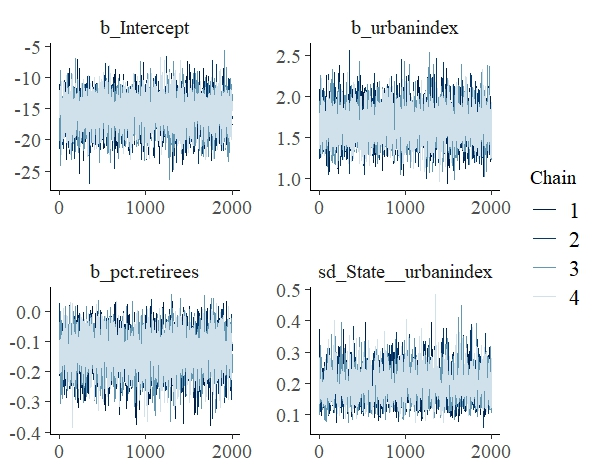
\includegraphics[scale = 1.25]{trace_plots/trace_model1.jpeg}

\begin{figure}[h!]
	\centering
	\caption{Trace plots for Model 1, all parameters; 2000 sampling iterations}
	\label{fig:trace_mod1_append}
	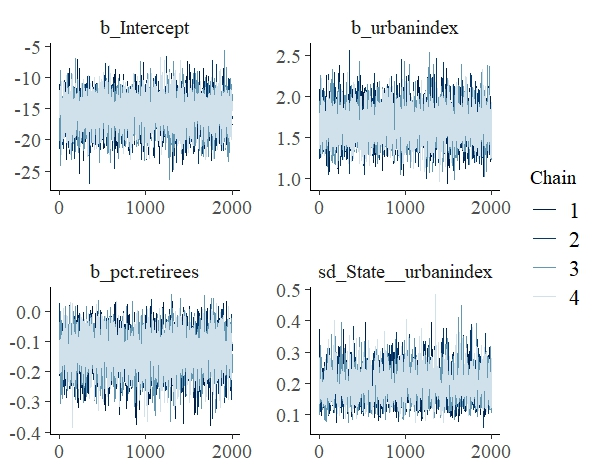
\includegraphics[width=0.8\textwidth]{trace_plots/trace_model1.jpeg}
\end{figure}


%Model 2:
%
%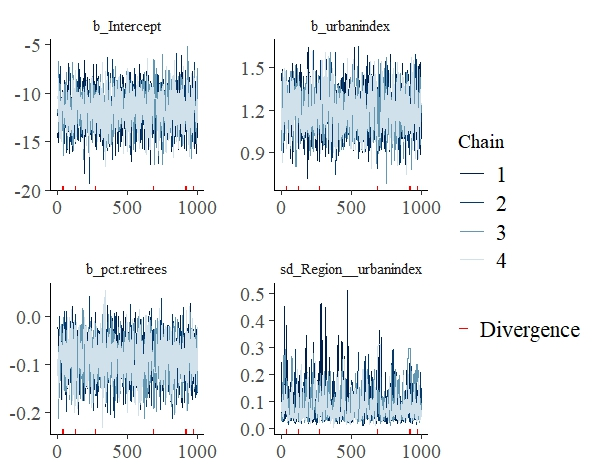
\includegraphics[scale = 1.4]{trace_plots/trace_model2.jpeg}


\begin{figure}[h!]
	\centering
	\caption{Trace plots for Model 2, all parameters; 2000 sampling iterations}
	\label{fig:trace_mod2_append}
	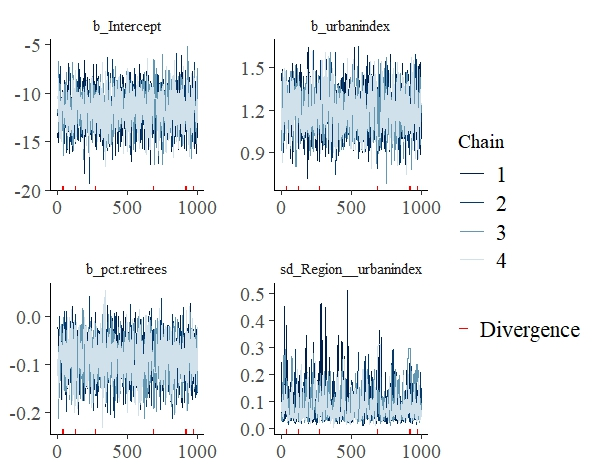
\includegraphics[width=0.8\textwidth]{trace_plots/trace_model2.jpeg}
\end{figure}

%Model 3 Pt 1:
%
%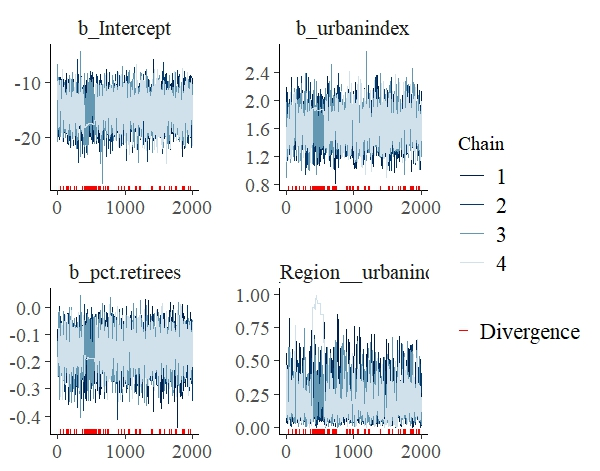
\includegraphics[scale = 1.25]{trace_plots/trace_model3_part1.jpeg}
%
%
%Model 3 Pt 2: 
%
%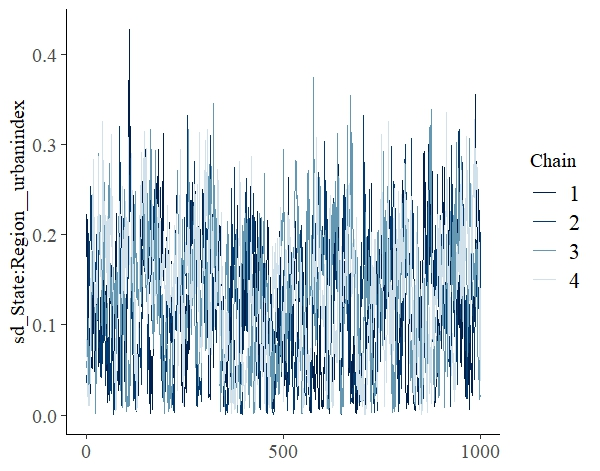
\includegraphics[scale = 1.25]{trace_plots/trace_model3_part2.jpeg}


\begin{figure}
	\centering
	\caption{Trace plots for Model 3, all parameters; 2000 sampling iterations}
	\label{fig:trace_mod3_append}
	\begin{subfigure}{\textwidth}
		\centering
		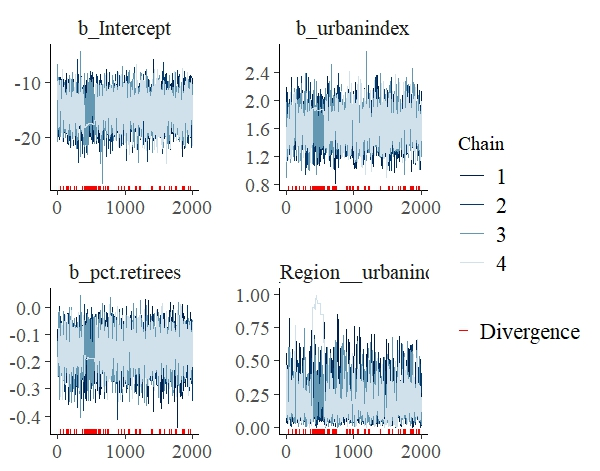
\includegraphics[width=0.8\textwidth]{trace_plots/trace_model3_part1.jpeg}
%		\caption{Caption for Figure 1}
%		\label{fig:fig1}
	\end{subfigure}
	
	\vspace{0.5em} % Adjust space between figures
	
	\begin{subfigure}{\textwidth}
		\centering
		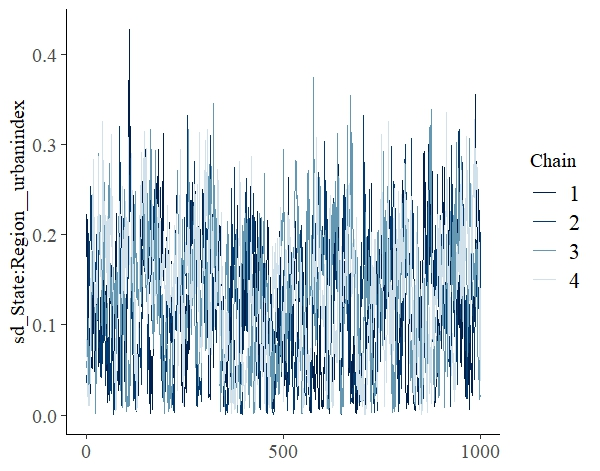
\includegraphics[width=0.5\textwidth]{trace_plots/trace_model3_part2}
%		\caption{Caption for Figure 2}
%		\label{fig:fig2}
	\end{subfigure}
	
\end{figure}




%Model 4 Pt 1:
%
%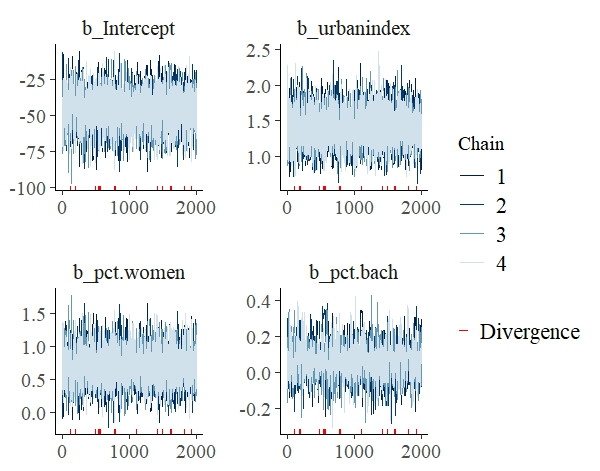
\includegraphics[scale = 1.3]{trace_plots/trace_model4_part1.jpeg}
%
%
%Model 4 Pt 2: 
%
%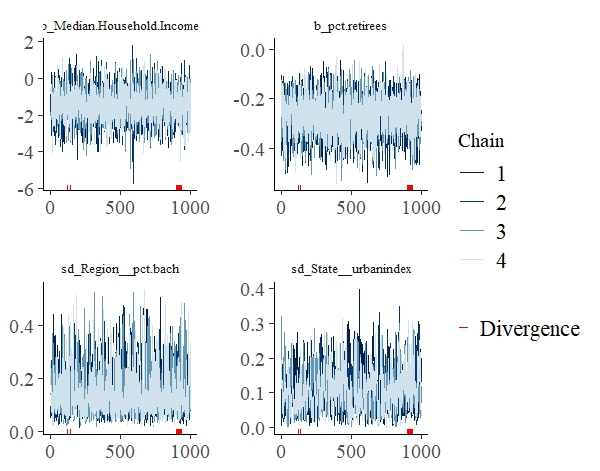
\includegraphics[scale = 1.3]{trace_plots/trace_model4_part2.jpeg}
%
%Model 4 Pt 3: 
%
%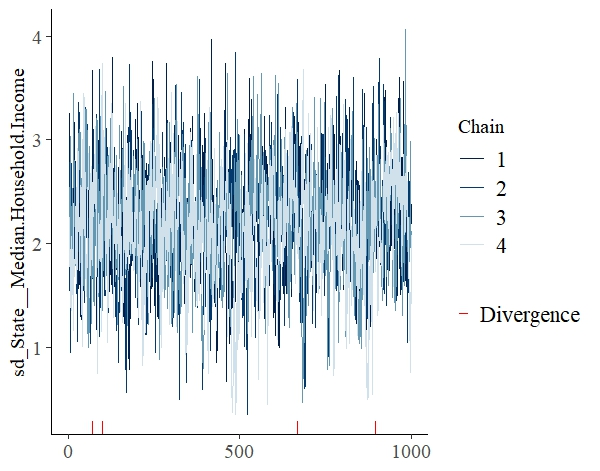
\includegraphics[scale = 1.4]{trace_plots/trace_model4_part3.jpeg}


\begin{figure}
	\centering
	\caption{Trace plots for Model 4, all parameters; 2000 sampling iterations}
	\label{fig:trace_mod4_append}
	\begin{subfigure}{\textwidth}
		\centering
		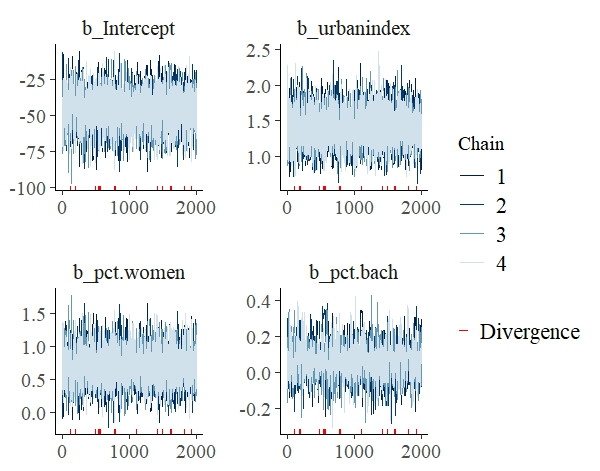
\includegraphics[width=0.7\textwidth]{trace_plots/trace_model4_part1.jpeg}
		%		\caption{Caption for Figure 1}
		%		\label{fig:fig1}
	\end{subfigure}
	
	\vspace{0.5em} % Adjust space between figures
	
	\begin{subfigure}{\textwidth}
		\centering
		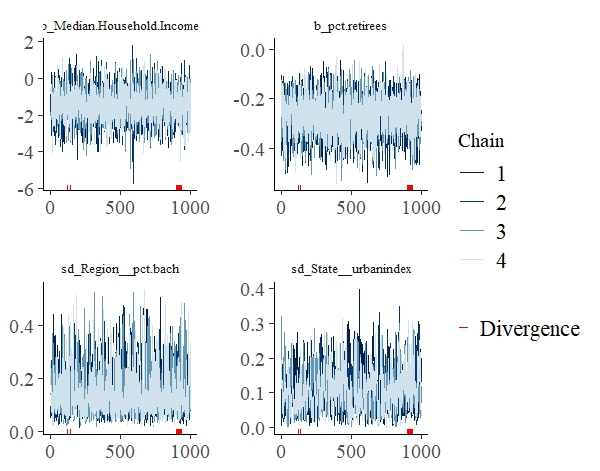
\includegraphics[width=0.7\textwidth]{trace_plots/trace_model4_part2}
		%		\caption{Caption for Figure 2}
		%		\label{fig:fig2}
	\end{subfigure}
	
	\vspace{0.5em} % Adjust space between figures
	
	\begin{subfigure}{\textwidth}
		\centering
		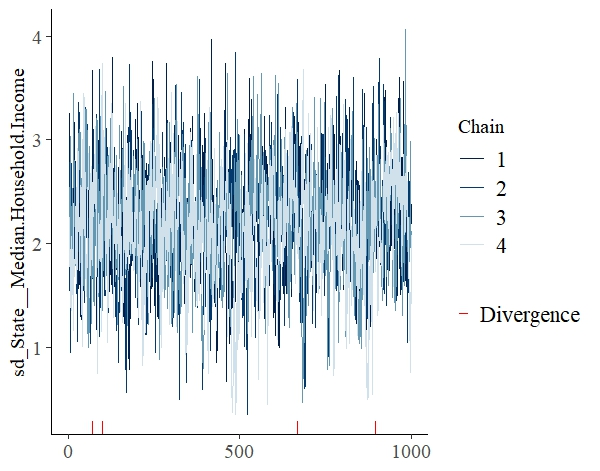
\includegraphics[width=0.4\textwidth]{trace_plots/trace_model4_part3}
		%		\caption{Caption for Figure 2}
		%		\label{fig:fig2}
	\end{subfigure}
	
\end{figure}


\clearpage
\FloatBarrier
\subsection*{Model Estimates}

\begin{table}[h!]
	\centering
	\caption{Parameter estimates obtained by Model 1 with all 435 observations, 4 chains, 4000 iterations (2000 warmup, 2000 sampling)}
	\label{tab:model1}
	 \begin{adjustbox}{max width=\textwidth}
	\begin{tabular}{rccccccc}
		\hline
		& Estimate & Est.Error & l-95\% CI & u-95\% CI & Rhat & Bulk\_ESS & Tail\_ESS \\ 
		\hline
		\multicolumn{8}{l}{Regression Coefficients:} \\
		Intercept & -15.75 & 2.63 & -20.96 & -10.73 & 1.00 & 7397.71 & 6010.33 \\ 
		urbanindex & 1.66 & 0.21 & 1.28 & 2.10 & 1.00 & 5191.43 & 5331.31 \\ 
		pct.retirees & -0.14 & 0.06 & -0.27 & -0.02 & 1.00 & 6086.48 & 5724.70 \\
		\midrule
		\multicolumn{8}{l}{Multilevel Hyperparameters: State (Number of levels: 50)}                       \\ 
		sd(urbanindex) & 0.19 & 0.05 & 0.11 & 0.30 & 1.00 & 1569.53 & 3108.00 \\ 
		\hline
	\end{tabular}
		\end{adjustbox}
\end{table}


\begin{table}[h!]
	\centering
	\caption{Parameter estimates obtained by Model 2 with all 435 observations, 4 chains, 4000 iterations (2000 warmup, 2000 sampling)}
	\label{tab:model2}
		 \begin{adjustbox}{max width=\textwidth}
	\begin{tabular}{rccccccc}
		\hline
		               & Estimate & Est.Error & l-95\% CI & u-95\% CI & Rhat & Bulk\_ESS & Tail\_ESS \\
		               \hline
 \multicolumn{8}{l}{Regression Coefficients:} \\
		     Intercept &   -12.01 &      1.78 &    -15.58 &     -8.60 & 1.00 &   2892.71 &   3356.25 \\
		    urbanindex &     1.22 &      0.15 &      0.95 &      1.53 & 1.00 &   1294.59 &    473.21 \\
		  pct.retirees &    -0.09 &      0.04 &     -0.16 &     -0.01 & 1.00 &   4773.23 &   4217.12 \\
		  \midrule
		  \multicolumn{8}{l}{Multilevel Hyperparameters: Region (Number of levels: 4)}                       \\
		sd(urbanindex) &     0.09 &      0.06 &      0.02 &      0.27 & 1.00 &    892.96 &    465.15 \\ \hline
	\end{tabular}
	\end{adjustbox}
	
\end{table}


\begin{table}[h!]
	\centering
	\caption{Parameter estimates obtained by Model 3 with all 435 observations, 4 chains, 4000 iterations (2000 warmup, 2000 sampling)}
	\label{tab:model3}
	\begin{adjustbox}{max width=\textwidth}
	\begin{tabular}{rccccccc}
		\hline
		& Estimate & Est.Error & l-95\% CI & u-95\% CI & Rhat & Bulk\_ESS & Tail\_ESS \\ 
		\hline
		 \multicolumn{8}{l}{Regression Coefficients:} \\
		Intercept & -15.02 & 2.69 & -20.32 & -9.87 & 1.00 & 2837.78 & 5324.03 \\ 
		urbanindex & 1.64 & 0.23 & 1.21 & 2.10 & 1.00 & 2787.63 & 2875.43 \\ 
		pct.retirees & -0.16 & 0.06 & -0.29 & -0.04 & 1.00 & 5424.17 & 5097.97 \\
		\midrule
		\multicolumn{8}{l}{Multilevel Hyperparameters: Region (Number of levels: 4)} \\ 
		sd(urbanindex) & 0.21 & 0.16 & 0.03 & 0.67 & 1.01 & 348.01 & 120.67 \\ 
		\midrule
		\multicolumn{8}{l}{Region:State (Number of levels: 50)}  \\
		sd(urbanindex)1 & 0.19 & 0.05 & 0.11 & 0.29 & 1.00 & 1976.07 & 3875.21 \\ 
		\hline
	\end{tabular}
	\end{adjustbox}
	
\end{table}


\begin{table}[ht!]
	\centering
	\caption{Parameter estimates obtained by Model 4 with all 435 observations, 4 chains, 4000 iterations (2000 warmup, 2000 sampling)}
	\label{tab:model4}
	\begin{adjustbox}{max width=\textwidth}
	\begin{tabular}{rccccccc}
		\hline
		& Estimate & Est.Error & l-95\% CI & u-95\% CI & Rhat & Bulk\_ESS & Tail\_ESS \\ 
		\hline
				 \multicolumn{8}{l}{Regression Coefficients:} \\
		Intercept & -45.84 & 12.13 & -70.40 & -22.99 & 1.00 & 6668.56 & 5729.57 \\ 
		urbanindex & 1.41 & 0.24 & 0.95 & 1.90 & 1.00 & 7707.06 & 6016.13 \\ 
		pct.women & 0.70 & 0.26 & 0.21 & 1.24 & 1.00 & 6155.31 & 4936.03 \\ 
		pct.bach & 0.06 & 0.09 & -0.11 & 0.27 & 1.00 & 1593.83 & 662.43 \\ 
		Median.Household.Income & -1.43 & 0.87 & -3.12 & 0.25 & 1.00 & 6817.58 & 3411.18 \\ 
		pct.retirees & -0.26 & 0.08 & -0.42 & -0.12 & 1.00 & 6809.18 & 5806.15 \\
		\midrule
		\multicolumn{8}{l}{Multilevel Hyperparameters: Region (Number of levels: 4)} \\ 
		sd(pct.bach) & 0.15 & 0.09 & 0.04 & 0.39 & 1.00 & 1855.37 & 1959.66 \\
		\midrule
		\multicolumn{8}{l}{Multilevel Hyperparameters: State (Number of levels: 50)}                       \\  
		sd(urbanindex) & 0.08 & 0.06 & 0.00 & 0.21 & 1.00 & 866.41 & 1941.43 \\ 
		sd(Median.Household.Income) & 2.24 & 0.51 & 1.19 & 3.26 & 1.00 & 2627.23 & 2493.48 \\ 
		\hline
	\end{tabular}
	\end{adjustbox}
	
\end{table}

\begin{figure}[h!]
	\centering
	\caption{Conditional effects of \textit{Urban Index}, for Model 3; mean in blue, with 95\% credible intervals in gray, observations in black;  group level effects included}
	\label{fig:cond_eff_mod3}
	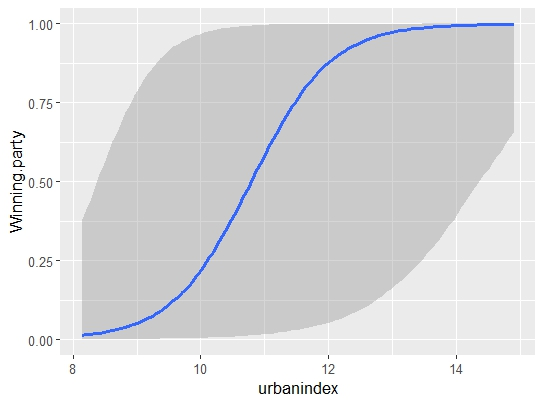
\includegraphics[width=0.6\textwidth]{results/cond_eff_urb_model3_groupeff.jpeg}
	
\end{figure}

\begin{figure}[h!]
	\centering
	\caption{Conditional effects of \textit{Urban Index}, for Model 4; mean in blue, with 95\% credible intervals in gray, observations in black;  group level effects included}
	\label{fig:cond_eff_mod4}
	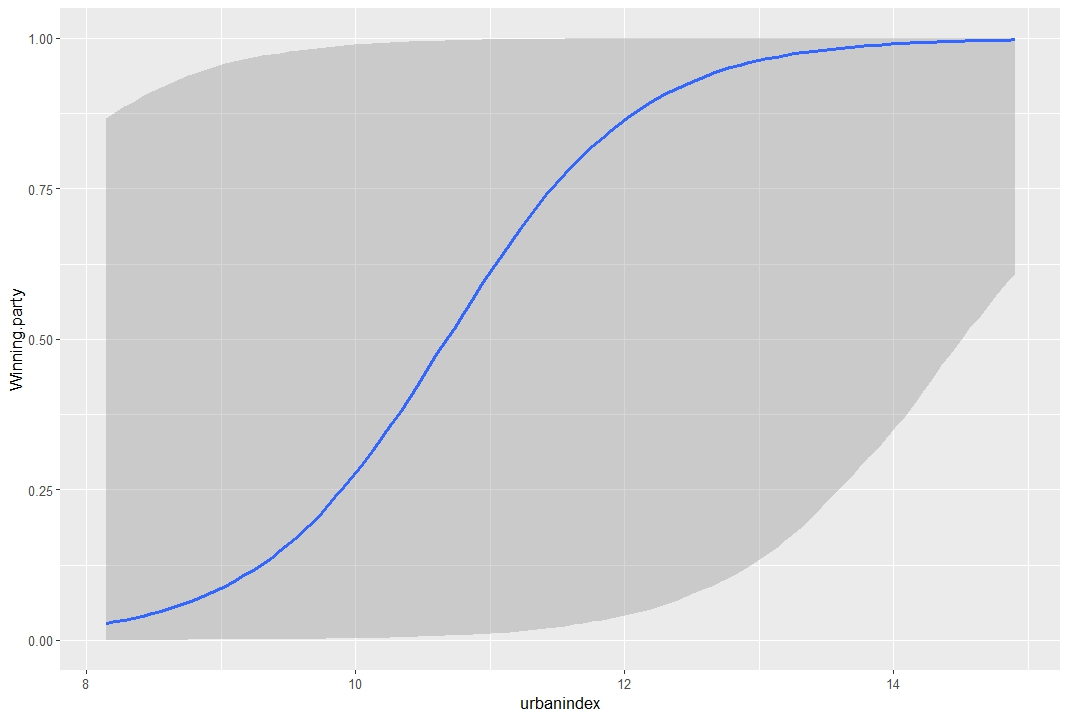
\includegraphics[width=0.6\textwidth]{results/cond_eff_urb_model4_groupeff_nopoints.jpeg}
	
\end{figure}



\FloatBarrier
\subsection*{Model Comparison Statistics}


\begin{figure}[h!]
	\centering
	\caption{Histograms of RMSE draws for all models}
	\label{fig:rmse}
	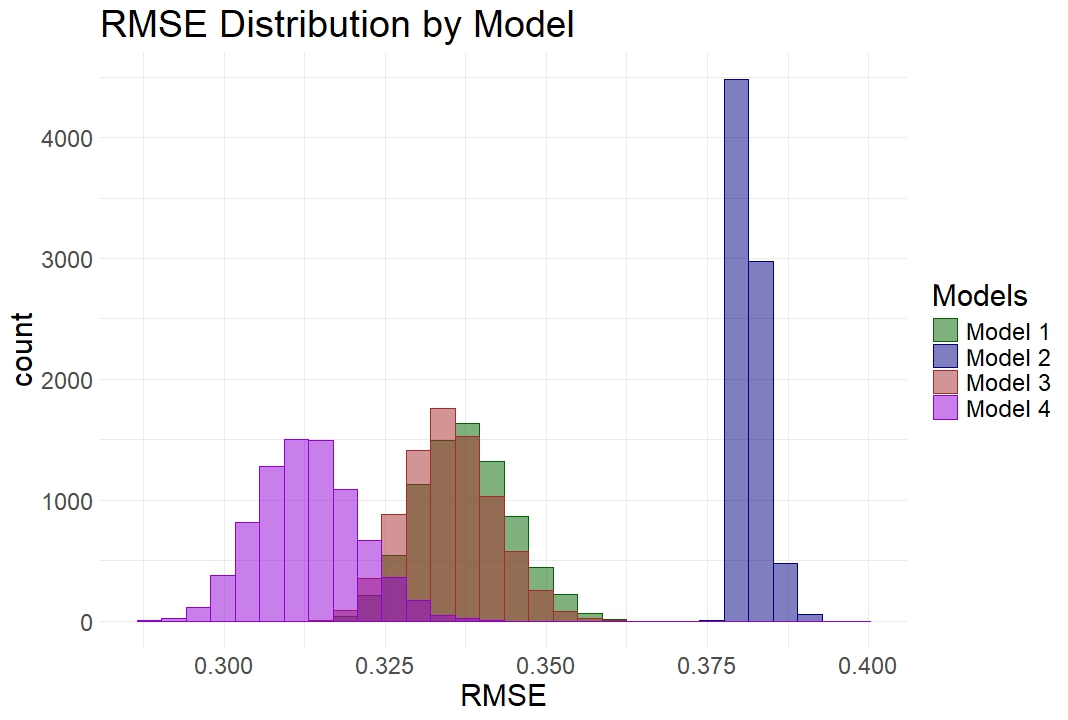
\includegraphics[width=0.6\textwidth]{model_comp_figures/RMSE_all.jpeg}
	
\end{figure}

\begin{figure}[h!]
	\centering
	\caption{Histograms of differences in Log-Likelihood Scores for each observation between all 4 models; black dotted line marks zero; red vertical line marks the mean of the difference between the corresponding models}
	\label{fig:ll_diff}
	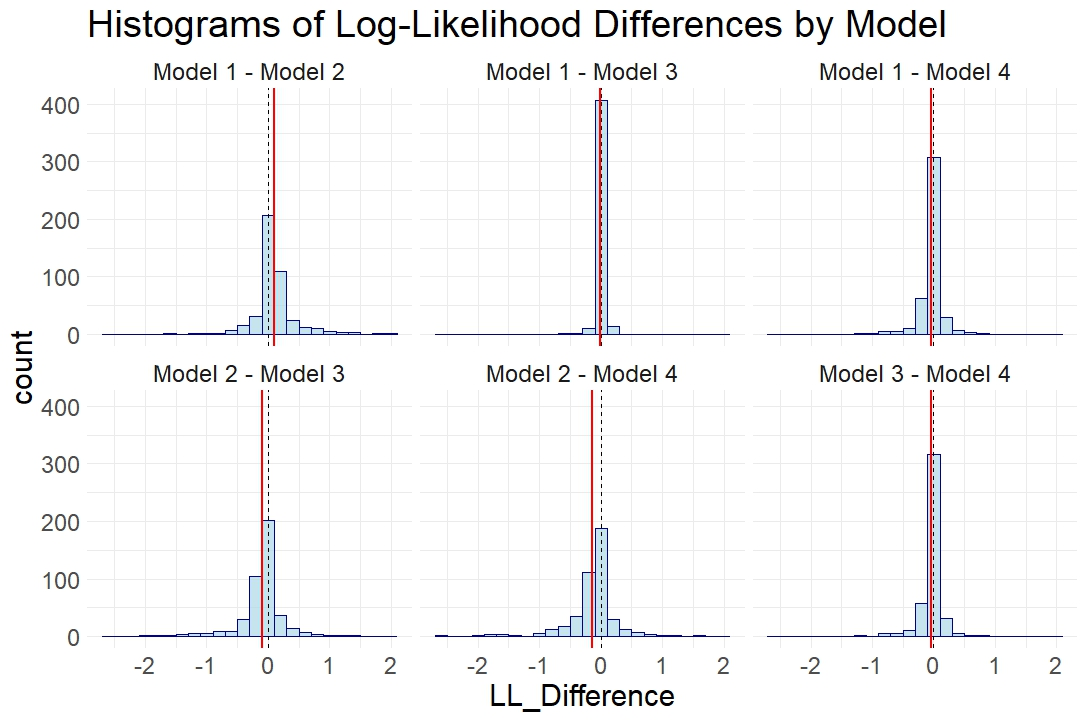
\includegraphics[width=0.8\textwidth]{model_comp_figures/LL_differences.jpeg}
	
\end{figure}


%\begin{figure}[h]
%	\centering
%	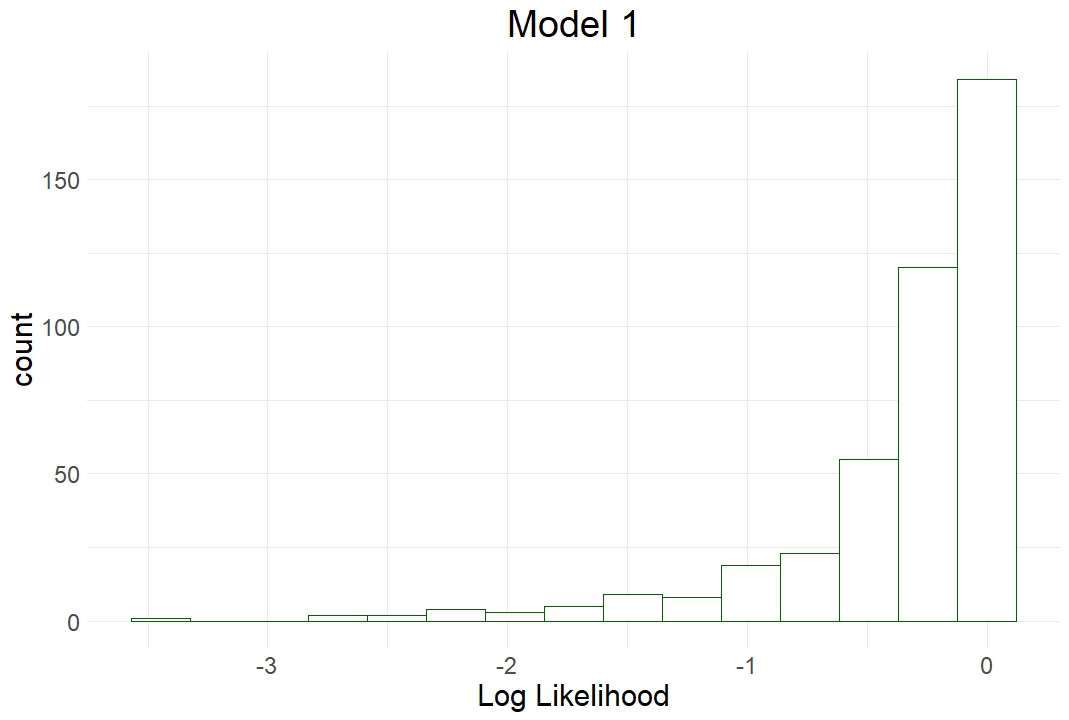
\includegraphics[width=0.8\textwidth]{model_comp_figures/LL_model1.jpeg}
%	\caption{}
%	\label{}
%\end{figure}
%
%\begin{figure}[h]
%	\centering
%	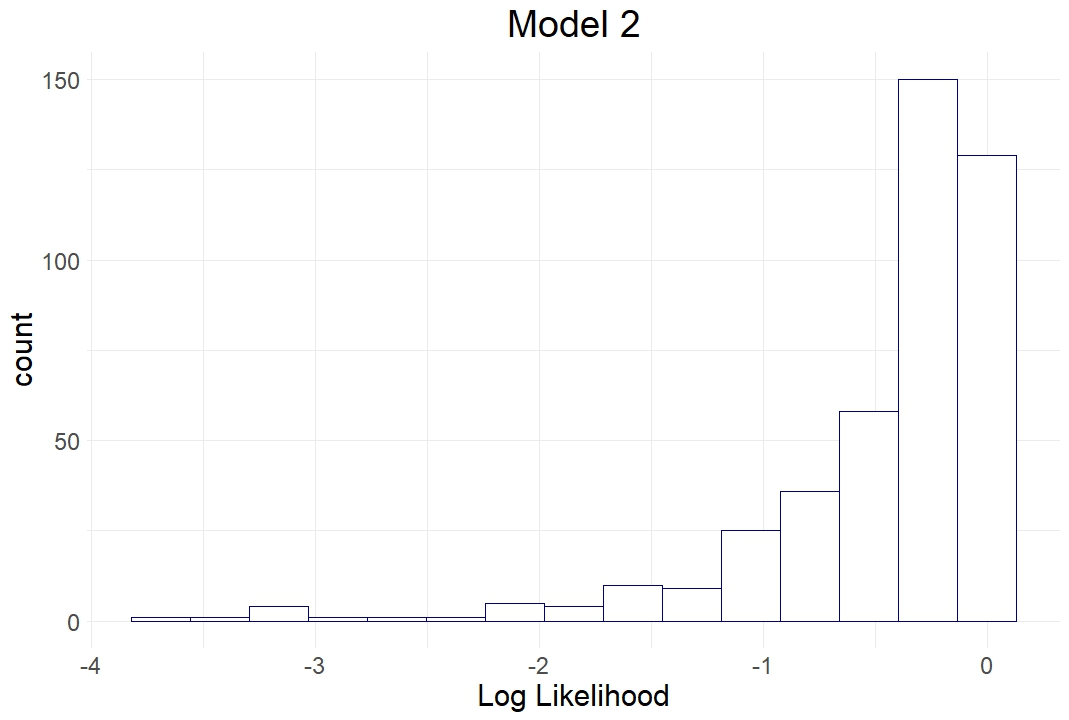
\includegraphics[width=0.8\textwidth]{model_comp_figures/LL_model2.jpeg}
%	\caption{}
%	\label{}
%\end{figure}
%
%\begin{figure}[h]
%	\centering
%	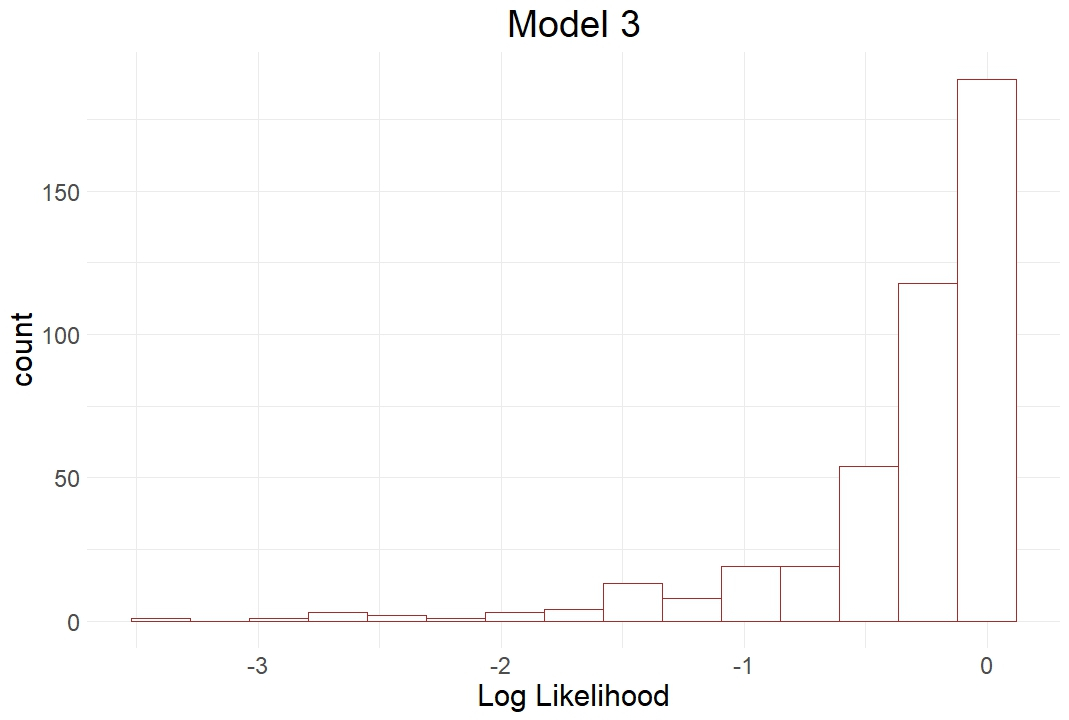
\includegraphics[width=0.8\textwidth]{model_comp_figures/LL_model3.jpeg}
%	\caption{}
%	\label{}
%\end{figure}
%
%\begin{figure}[h]
%	\centering
%	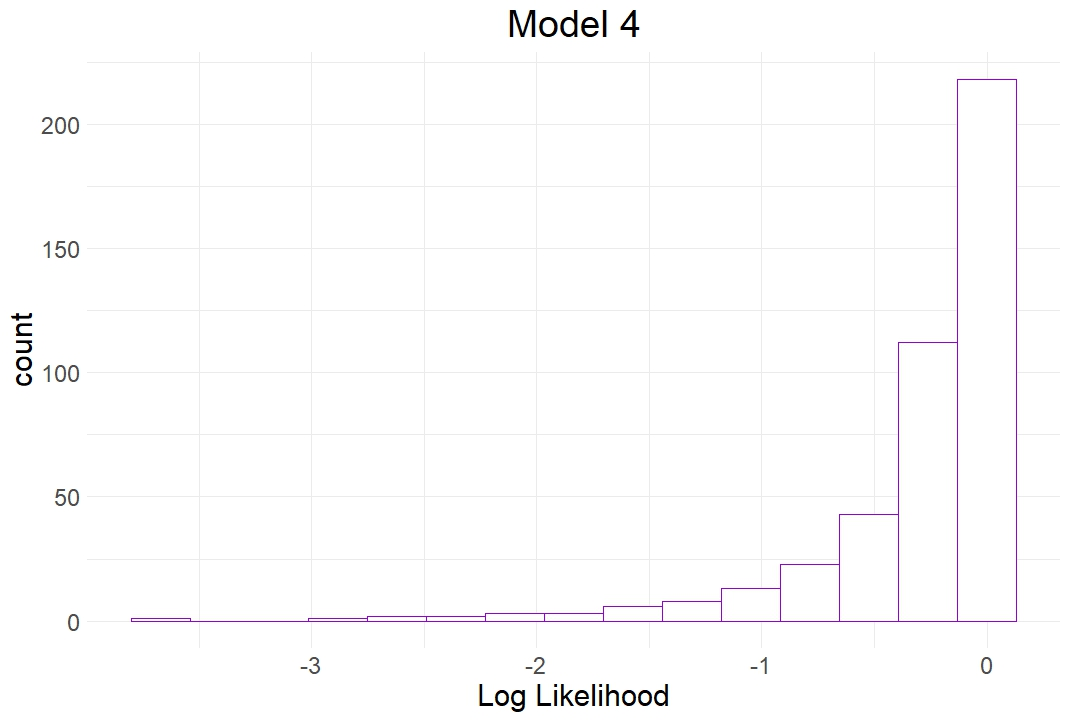
\includegraphics[width=0.8\textwidth]{model_comp_figures/LL_model4.jpeg}
%	\caption{}
%	\label{}
%\end{figure}



\begin{table}[ht!]
	\centering
	\caption{LOO statistics with moment matching}
	\begin{tabular}{rrrrrrrrr}
		\hline
		& elpd\_diff & se\_diff & elpd\_loo & se\_elpd\_loo & p\_loo & se\_p\_loo & looic & se\_looic \\ 
		\hline
		model4.final & 0.00 & 0.00 & -156.49 & 11.59 & 32.57 & 3.25 & 312.98 & 23.19 \\ 
		model3.final & -17.99 & 4.23 & -174.48 & 12.11 & 33.08 & 3.33 & 348.97 & 24.22 \\ 
		model1.final & -20.32 & 4.60 & -176.81 & 12.08 & 33.34 & 3.42 & 353.61 & 24.17 \\ 
		model2.final & -45.87 & 8.39 & -202.36 & 12.25 & 6.19 & 0.58 & 404.71 & 24.50 \\ 
		\hline
	\end{tabular}

\end{table}






\FloatBarrier
\subsection*{Prior Sensitivity Analysis}
\begin{table}[h]
    \centering
    \caption{Prior Sensitivity Results for Model 1}
    \label{tab:Prior Sensitivity Results for Model 1}
    \begin{tabular}{l|ccccc}
        \hline
        Coefficient    & Prior Set 1 & Prior Set 2 & Prior Set 3 & Prior Set 4 & Prior Set 5 \\
        \hline
        Intercept      & -12.0110 & -11.8230 & -12.1806 & -11.9011 & -12.1806 \\
        Urban Index    & 1.2167 & 1.2005 & 1.2311 & 1.2047 & 1.2311 \\
        Pct. Retirees  & -0.0861 & -0.0882 & -0.0843 & -0.0873 & -0.0843 \\
        SD Urban       & 0.19    & 0.19    & 0.2     & 0.19    & 0.2     \\
        \hline
        \hline
    \end{tabular}

\end{table}

\begin{table}[h]
    \centering
    \caption{Prior Sensitivity Results for Model 3}
    \label{tab:Prior Sensitivity Results for Model 3}
    \begin{tabular}{l|ccccc}
        \hline
        Coefficient    & Prior Set 1 & Prior Set 2 & Prior Set 3 & Prior Set 4 & Prior Set 5 \\
        \hline
        Intercept      & -15.0192 & -14.9687 & -15.7396 & -14.9113 & -15.7476 \\
        Urban Index    & 1.6368 & 1.6327 & 1.7139 & 1.6312 & 1.7189 \\
        Pct. Retirees  & -0.1599 & -0.1596 & -0.1577 & -0.1606 & -0.1568 \\
        SD Urban       & 0.1    & 0.1    & 0.1     & 0.1    & 0.1     \\
        \hline
    \end{tabular}
    
\end{table}






\FloatBarrier

\clearpage
\newpage
\printbibliography

\end{document}
